\documentclass
{article}
\usepackage[margin=1in]{geometry}

\usepackage{authblk}

\title{Constraint Optimization of MicroPlate Designs:\\supplementary materials}
\author{Ramiz Gindullin\textsuperscript{\rm 1}, Mar\'ia~Andre\'ina Francisco~Rodr\'iguez\textsuperscript{\rm 1}}
\affil{\small
    \textsuperscript{\rm 1}Uppsala University, Sweden\\
    {Ramiz.Gindullin@it.uu.se}, {Maria.Andreina.Francisco@it.uu.se}
}


%%%%%%%%%%%%%%%%%%%%%%%%%%%%%%%%%%%%%%%%%%%%%%%%%%%%%%

\input{0c_packages}
\input{0c_macros}

\begin{document}


\maketitle

\begin{abstract}
    We present detailed results of computational experiments of the paper published in the proceedings of the 2026 AAAI conference~\cite{gindullin26compd}.
\end{abstract}

\section*{Overview}

Here we provide the complete list of figures and tables containing results of replicated experiments from the paper~\cite{plaid2023} (we will use `the PLAID paper' for brevity):

\begin{itemize}
    \item Figures~\ref{fig:dose_response_paper} and \ref{fig:screening} correspond to Figures~2 and 3 (resp.) of the PLAID paper;

    \item Figures and tables in \ref{sec:dose-response} and \ref{sec:screening} correspond to Figures~1--24 (resp.) from the supplementary materials of the PLAID paper, with some additions (mostly, in detailed tables).

\end{itemize}

\bibliographystyle{plain}
\bibliography{compd_bibliography}

\clearpage

% Compact paper figures (one per experiment type) — kept here for a quick summary.
\begin{figure*}
  \centering

  %% Row 1 — example dose-response curves (one panel per layout)
  \begin{subfigure}[t]{0.315\textwidth}
    \centering
    \caption{Random (3 replicates)}
    \includegraphics[width=\linewidth]{figures/plate_layout_rand_02.npy_compound_4-right-half.png}
    \label{fig:dr-curves-half-right}
  \end{subfigure}
  \hfill
  \begin{subfigure}[t]{0.315\textwidth}
    \centering
    \caption{PLAID (3 replicates)}
    \includegraphics[width=\linewidth]{figures/plate_layout_20-12-8-3_01.npy_compound_4-right-half.png}
  \end{subfigure}
  \hfill
  \begin{subfigure}[t]{0.315\textwidth}
    \centering
    \caption{COMPD (3 replicates)}
    \includegraphics[width=\linewidth]{figures/plate_layout_40-12-8-3_01.npy_compound_4-right-half.png}
  \end{subfigure}

  \vspace{0.5em}

  %% Row 2 — residuals and d_max difference
  \begin{subfigure}[t]{0.49\textwidth}
    \centering
    \caption{Residuals}
    \includegraphics[width=\linewidth]{figures/residuals-1-2-3-8doses-dil8-half-columns-neg-controls-0.4_paper.png}
    \label{fig:residuals-8-doses-half-right}
  \end{subfigure}
  \hfill
  \begin{subfigure}[t]{0.49\textwidth}
    \centering
    \caption{Mean absolute $d$ (max) difference}
    \includegraphics[width=\linewidth]{figures/dose-response-d_diff-1-2-3-8doses-dil8-right-half-neg-controls-0.4_paper.png}
  \end{subfigure}

  \vspace{0.5em}

  %% Row 3 — IC50 / EC50 estimates
  \begin{subfigure}[t]{0.49\textwidth}
    \centering
    \caption{Relative $\text{IC}_{50}$/$\text{EC}_{50}$}
    \includegraphics[width=\linewidth]{figures/dose-response-relic50-1-2-3-8doses-dil8-half-columns-neg-controls-0.4_paper.png}
    \label{fig:relic50-8-doses-half-right}
  \end{subfigure}
  \hfill
  \begin{subfigure}[t]{0.49\textwidth}
    \centering
    \caption{Absolute $\text{IC}_{50}$/$\text{EC}_{50}$}
    \includegraphics[width=\linewidth]{figures/dose-response-absic50-1-2-3-8doses-dil8-right-half-neg-controls-0.4_paper.png}
    \label{fig:absic50-8-doses-half-right}
  \end{subfigure}

  \caption{Comparison between expected and obtaine¸d values for dose-response
    curves with $8$ doses, $1$, $2$, or $3$ replicates, $20$ negative controls
    on a 384-well plate, and strong plate effects with a linear relationship to
    column number on the right side of the plate.
    * indicates ${p<10^{-4}}$,
    ** indicates ${p<10^{-12}}$,
    *** indicates ${p<10^{-43}}$.}
  \label{fig:dose_response_paper}
\end{figure*}


%%% Local Variables:
%%% mode: latex
%%% TeX-master: "main.tex"
%%% End:
\input{tikz-figures/screening_data__paper}
%%============================================================
\clearpage
\section{Dose-response experiments}\label{sec:dose-response}
%%============================================================

% AUTO-GENERATED by run_dose_response_benchmark.py -- DO NOT EDIT.
% Regenerate with:  python run_dose_response_benchmark.py --stage tables
%

\subsection{\emph{bowl-shaped} plate effects (bowl (negatives unaffected))}


\subsubsection{$d_{\max}$ errors}

\begin{figure*}[!htbp]
  \centering
  \begin{subfigure}[c]{0.05\textwidth}
    ~
  \end{subfigure}
  %
  \begin{subfigure}[c]{0.40\textwidth}
    \centering
    ~~\textbf{Mild plate effects}
  \end{subfigure}
  %
  \begin{subfigure}[c]{0.40\textwidth}
    \centering
    ~~\textbf{Strong plate effects}
  \end{subfigure}

  \begin{subfigure}[c]{0.05\textwidth}
    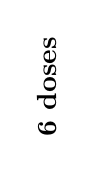
\begin{tikzpicture}
      \node[rotate=90] {\textbf{6 doses}};
    \end{tikzpicture}
  \end{subfigure}
  %
  \begin{subfigure}[c]{0.40\textwidth}
    \includegraphics[width=\textwidth]{figures/dose-response-d_diff-1-2-3-6doses-dil18-bowl-0.055.png}
  \end{subfigure}
  %
  \begin{subfigure}[c]{0.40\textwidth}
    \centering
    \includegraphics[width=\textwidth]{figures/dose-response-d_diff-1-2-3-6doses-dil18-bowl-0.085.png}
  \end{subfigure}

  \begin{subfigure}[c]{0.05\textwidth}
    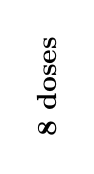
\begin{tikzpicture}
      \node[rotate=90] {\textbf{8 doses}};
    \end{tikzpicture}
  \end{subfigure}
  %
  \begin{subfigure}[c]{0.40\textwidth}
    \includegraphics[width=\textwidth]{figures/dose-response-d_diff-1-2-3-8doses-dil8-bowl-0.055.png}
  \end{subfigure}
  %
  \begin{subfigure}[c]{0.40\textwidth}
    \centering
    \includegraphics[width=\textwidth]{figures/dose-response-d_diff-1-2-3-8doses-dil8-bowl-0.085.png}
  \end{subfigure}

  \begin{subfigure}[c]{0.05\textwidth}
    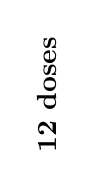
\begin{tikzpicture}
      \node[rotate=90] {\textbf{12 doses}};
    \end{tikzpicture}
  \end{subfigure}
  %
  \begin{subfigure}[c]{0.40\textwidth}
    \includegraphics[width=\textwidth]{figures/dose-response-d_diff-1-2-3-12doses-dil4-bowl-0.055.png}
  \end{subfigure}
  %
  \begin{subfigure}[c]{0.40\textwidth}
    \centering
    \includegraphics[width=\textwidth]{figures/dose-response-d_diff-1-2-3-12doses-dil4-bowl-0.085.png}
  \end{subfigure}

  \caption{Mean absolute difference between expected and obtained heights ($d_{\max}$) for dose-response curves using various numbers of doses, replicates, and \emph{bowl-shaped} plate-effect strengths. The 4PL sigmoid curves were fitted using compound data and 4 negative controls such that their mean was equal to the mean of the 20 negative controls on the plate. *** indicates $p\leq10^{-43}$.}
\end{figure*}

\begin{table}[H]
  \caption{%
    $d_{max}$ error overview for \emph{bowl-shaped} plate-effect strengths. Values are mean absolute differences in fitted $d_{max}$ across compounds. Best (lowest) value per row is \textbf{bolded}.
  }
  \label{tab:dr-overview-dmax-bowl}
  \centering
  \input{tables/dr-overview-dmax-bowl}
\end{table}


\clearpage
\subsubsection{Relative IC$_{50}$/EC$_{50}$ errors}

\begin{figure*}[!htbp]
  \centering
  \begin{subfigure}[c]{0.05\textwidth}
    ~
  \end{subfigure}
  %
  \begin{subfigure}[c]{0.40\textwidth}
    \centering
    ~~\textbf{Mild plate effects}
  \end{subfigure}
  %
  \begin{subfigure}[c]{0.40\textwidth}
    \centering
    ~~\textbf{Strong plate effects}
  \end{subfigure}

  \begin{subfigure}[c]{0.05\textwidth}
    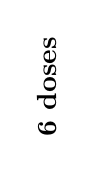
\begin{tikzpicture}
      \node[rotate=90] {\textbf{6 doses}};
    \end{tikzpicture}
  \end{subfigure}
  %
  \begin{subfigure}[c]{0.40\textwidth}
    \includegraphics[width=\textwidth]{figures/dose-response-relic50-1-2-3-6doses-dil18-bowl-0.055.png}
  \end{subfigure}
  %
  \begin{subfigure}[c]{0.40\textwidth}
    \centering
    \includegraphics[width=\textwidth]{figures/dose-response-relic50-1-2-3-6doses-dil18-bowl-0.085.png}
  \end{subfigure}

  \begin{subfigure}[c]{0.05\textwidth}
    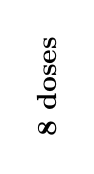
\begin{tikzpicture}
      \node[rotate=90] {\textbf{8 doses}};
    \end{tikzpicture}
  \end{subfigure}
  %
  \begin{subfigure}[c]{0.40\textwidth}
    \includegraphics[width=\textwidth]{figures/dose-response-relic50-1-2-3-8doses-dil8-bowl-0.055.png}
  \end{subfigure}
  %
  \begin{subfigure}[c]{0.40\textwidth}
    \centering
    \includegraphics[width=\textwidth]{figures/dose-response-relic50-1-2-3-8doses-dil8-bowl-0.085.png}
  \end{subfigure}

  \begin{subfigure}[c]{0.05\textwidth}
    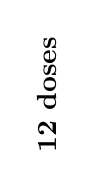
\begin{tikzpicture}
      \node[rotate=90] {\textbf{12 doses}};
    \end{tikzpicture}
  \end{subfigure}
  %
  \begin{subfigure}[c]{0.40\textwidth}
    \includegraphics[width=\textwidth]{figures/dose-response-relic50-1-2-3-12doses-dil4-bowl-0.055.png}
  \end{subfigure}
  %
  \begin{subfigure}[c]{0.40\textwidth}
    \centering
    \includegraphics[width=\textwidth]{figures/dose-response-relic50-1-2-3-12doses-dil4-bowl-0.085.png}
  \end{subfigure}

  \caption{Relative IC$_{50}$/EC$_{50}$ error for dose-response curves using various numbers of doses, replicates, and \emph{bowl-shaped} plate-effect strengths. *** indicates $p\leq10^{-43}$.}
\end{figure*}

\begin{table}[H]
  \caption{%
    Relative IC$_{50}$/EC$_{50}$ MSE overview for \emph{bowl-shaped} plate-effect strengths. Best (lowest) value per row is \textbf{bolded}.
  }
  \label{tab:dr-overview-rel-ic50-bowl}
  \centering
  \input{tables/dr-overview-rel-ic50-bowl}
\end{table}


\clearpage
\subsubsection{Absolute IC$_{50}$/EC$_{50}$ errors}

\begin{figure*}[!htbp]
  \centering
  \begin{subfigure}[c]{0.05\textwidth}
    ~
  \end{subfigure}
  %
  \begin{subfigure}[c]{0.40\textwidth}
    \centering
    ~~\textbf{Mild plate effects}
  \end{subfigure}
  %
  \begin{subfigure}[c]{0.40\textwidth}
    \centering
    ~~\textbf{Strong plate effects}
  \end{subfigure}

  \begin{subfigure}[c]{0.05\textwidth}
    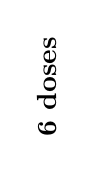
\begin{tikzpicture}
      \node[rotate=90] {\textbf{6 doses}};
    \end{tikzpicture}
  \end{subfigure}
  %
  \begin{subfigure}[c]{0.40\textwidth}
    \includegraphics[width=\textwidth]{figures/dose-response-absic50-1-2-3-6doses-dil18-bowl-0.055.png}
  \end{subfigure}
  %
  \begin{subfigure}[c]{0.40\textwidth}
    \centering
    \includegraphics[width=\textwidth]{figures/dose-response-absic50-1-2-3-6doses-dil18-bowl-0.085.png}
  \end{subfigure}

  \begin{subfigure}[c]{0.05\textwidth}
    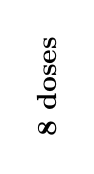
\begin{tikzpicture}
      \node[rotate=90] {\textbf{8 doses}};
    \end{tikzpicture}
  \end{subfigure}
  %
  \begin{subfigure}[c]{0.40\textwidth}
    \includegraphics[width=\textwidth]{figures/dose-response-absic50-1-2-3-8doses-dil8-bowl-0.055.png}
  \end{subfigure}
  %
  \begin{subfigure}[c]{0.40\textwidth}
    \centering
    \includegraphics[width=\textwidth]{figures/dose-response-absic50-1-2-3-8doses-dil8-bowl-0.085.png}
  \end{subfigure}

  \begin{subfigure}[c]{0.05\textwidth}
    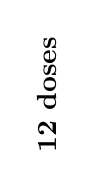
\begin{tikzpicture}
      \node[rotate=90] {\textbf{12 doses}};
    \end{tikzpicture}
  \end{subfigure}
  %
  \begin{subfigure}[c]{0.40\textwidth}
    \includegraphics[width=\textwidth]{figures/dose-response-absic50-1-2-3-12doses-dil4-bowl-0.055.png}
  \end{subfigure}
  %
  \begin{subfigure}[c]{0.40\textwidth}
    \centering
    \includegraphics[width=\textwidth]{figures/dose-response-absic50-1-2-3-12doses-dil4-bowl-0.085.png}
  \end{subfigure}

  \caption{Absolute IC$_{50}$/EC$_{50}$ error for dose-response curves using various numbers of doses, replicates, and \emph{bowl-shaped} plate-effect strengths. *** indicates $p\leq10^{-43}$.}
\end{figure*}

\begin{table}[H]
  \caption{%
    Absolute IC$_{50}$/EC$_{50}$ error overview for \emph{bowl-shaped} plate-effect strengths. Values are mean squared absolute IC$_{50}$/EC$_{50}$ estimation errors across compounds. Best (lowest) value per row is \textbf{bolded}.
  }
  \label{tab:dr-overview-abs-ic50-bowl}
  \centering
  \input{tables/dr-overview-abs-ic50-bowl}
\end{table}


\clearpage
\subsubsection{Residuals}

\begin{figure*}[!htbp]
  \centering
  \begin{subfigure}[c]{0.05\textwidth}
    ~
  \end{subfigure}
  %
  \begin{subfigure}[c]{0.40\textwidth}
    \centering
    ~~\textbf{Mild plate effects}
  \end{subfigure}
  %
  \begin{subfigure}[c]{0.40\textwidth}
    \centering
    ~~\textbf{Strong plate effects}
  \end{subfigure}

  \begin{subfigure}[c]{0.05\textwidth}
    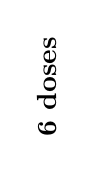
\begin{tikzpicture}
      \node[rotate=90] {\textbf{6 doses}};
    \end{tikzpicture}
  \end{subfigure}
  %
  \begin{subfigure}[c]{0.40\textwidth}
    \includegraphics[width=\textwidth]{figures/residuals-1-2-3-6doses-dil18-bowl-0.055.png}
  \end{subfigure}
  %
  \begin{subfigure}[c]{0.40\textwidth}
    \centering
    \includegraphics[width=\textwidth]{figures/residuals-1-2-3-6doses-dil18-bowl-0.085.png}
  \end{subfigure}

  \begin{subfigure}[c]{0.05\textwidth}
    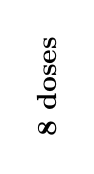
\begin{tikzpicture}
      \node[rotate=90] {\textbf{8 doses}};
    \end{tikzpicture}
  \end{subfigure}
  %
  \begin{subfigure}[c]{0.40\textwidth}
    \includegraphics[width=\textwidth]{figures/residuals-1-2-3-8doses-dil8-bowl-0.055.png}
  \end{subfigure}
  %
  \begin{subfigure}[c]{0.40\textwidth}
    \centering
    \includegraphics[width=\textwidth]{figures/residuals-1-2-3-8doses-dil8-bowl-0.085.png}
  \end{subfigure}

  \begin{subfigure}[c]{0.05\textwidth}
    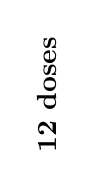
\begin{tikzpicture}
      \node[rotate=90] {\textbf{12 doses}};
    \end{tikzpicture}
  \end{subfigure}
  %
  \begin{subfigure}[c]{0.40\textwidth}
    \includegraphics[width=\textwidth]{figures/residuals-1-2-3-12doses-dil4-bowl-0.055.png}
  \end{subfigure}
  %
  \begin{subfigure}[c]{0.40\textwidth}
    \centering
    \includegraphics[width=\textwidth]{figures/residuals-1-2-3-12doses-dil4-bowl-0.085.png}
  \end{subfigure}

  \caption{Residuals (MSE between expected and obtained responses) for dose-response simulations using various numbers of doses, replicates, and \emph{bowl-shaped} plate-effect strengths. *** indicates $p\leq10^{-43}$.}
\end{figure*}

\begin{table}[H]
  \caption{%
    Residual MSE overview for \emph{bowl-shaped} plate-effect strengths. Best (lowest) value per row is \textbf{bolded}.
  }
  \label{tab:dr-overview-residuals-bowl}
  \centering
  \input{tables/dr-overview-residuals-bowl}
\end{table}


\clearpage
\subsubsection{Fraction of poor fits (low $R^2$)}

\begin{figure*}[!htbp]
  \centering
  \begin{subfigure}[c]{0.05\textwidth}
    ~
  \end{subfigure}
  %
  \begin{subfigure}[c]{0.40\textwidth}
    \centering
    ~~\textbf{Mild plate effects}
  \end{subfigure}
  %
  \begin{subfigure}[c]{0.40\textwidth}
    \centering
    ~~\textbf{Strong plate effects}
  \end{subfigure}

  \begin{subfigure}[c]{0.05\textwidth}
    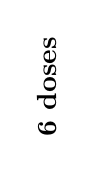
\begin{tikzpicture}
      \node[rotate=90] {\textbf{6 doses}};
    \end{tikzpicture}
  \end{subfigure}
  %
  \begin{subfigure}[c]{0.40\textwidth}
    \includegraphics[width=\textwidth]{figures/percentage-low-r2-curves-1-2-3-6doses-dil18-bowl-0.055.png}
  \end{subfigure}
  %
  \begin{subfigure}[c]{0.40\textwidth}
    \centering
    \includegraphics[width=\textwidth]{figures/percentage-low-r2-curves-1-2-3-6doses-dil18-bowl-0.085.png}
  \end{subfigure}

  \begin{subfigure}[c]{0.05\textwidth}
    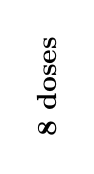
\begin{tikzpicture}
      \node[rotate=90] {\textbf{8 doses}};
    \end{tikzpicture}
  \end{subfigure}
  %
  \begin{subfigure}[c]{0.40\textwidth}
    \includegraphics[width=\textwidth]{figures/percentage-low-r2-curves-1-2-3-8doses-dil8-bowl-0.055.png}
  \end{subfigure}
  %
  \begin{subfigure}[c]{0.40\textwidth}
    \centering
    \includegraphics[width=\textwidth]{figures/percentage-low-r2-curves-1-2-3-8doses-dil8-bowl-0.085.png}
  \end{subfigure}

  \begin{subfigure}[c]{0.05\textwidth}
    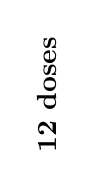
\begin{tikzpicture}
      \node[rotate=90] {\textbf{12 doses}};
    \end{tikzpicture}
  \end{subfigure}
  %
  \begin{subfigure}[c]{0.40\textwidth}
    \includegraphics[width=\textwidth]{figures/percentage-low-r2-curves-1-2-3-12doses-dil4-bowl-0.055.png}
  \end{subfigure}
  %
  \begin{subfigure}[c]{0.40\textwidth}
    \centering
    \includegraphics[width=\textwidth]{figures/percentage-low-r2-curves-1-2-3-12doses-dil4-bowl-0.085.png}
  \end{subfigure}

  \caption{Percentage of dose-response curves with low-quality ($R^2 < 80\%$) using various numbers of doses, replicates, and \emph{bowl-shaped} plate-effect strengths. The 4PL sigmoid curves were fitted using compound data and 4 negative controls such that their mean was equal to the mean of the 20 negative controls on the plate.}
\end{figure*}

\clearpage
\subsection{\emph{bowl-shaped} plate effects (bowl (negatives affected))}


\subsubsection{$d_{\max}$ errors}

\begin{figure*}[!htbp]
  \centering
  \begin{subfigure}[c]{0.05\textwidth}
    ~
  \end{subfigure}
  %
  \begin{subfigure}[c]{0.40\textwidth}
    \centering
    ~~\textbf{Mild plate effects}
  \end{subfigure}
  %
  \begin{subfigure}[c]{0.40\textwidth}
    \centering
    ~~\textbf{Strong plate effects}
  \end{subfigure}

  \begin{subfigure}[c]{0.05\textwidth}
    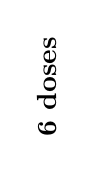
\begin{tikzpicture}
      \node[rotate=90] {\textbf{6 doses}};
    \end{tikzpicture}
  \end{subfigure}
  %
  \begin{subfigure}[c]{0.40\textwidth}
    \includegraphics[width=\textwidth]{figures/dose-response-d_diff-1-2-3-6doses-dil18-bowl-neg-controls-0.055.png}
  \end{subfigure}
  %
  \begin{subfigure}[c]{0.40\textwidth}
    \centering
    \includegraphics[width=\textwidth]{figures/dose-response-d_diff-1-2-3-6doses-dil18-bowl-neg-controls-0.085.png}
  \end{subfigure}

  \begin{subfigure}[c]{0.05\textwidth}
    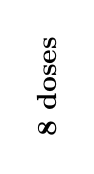
\begin{tikzpicture}
      \node[rotate=90] {\textbf{8 doses}};
    \end{tikzpicture}
  \end{subfigure}
  %
  \begin{subfigure}[c]{0.40\textwidth}
    \includegraphics[width=\textwidth]{figures/dose-response-d_diff-1-2-3-8doses-dil8-bowl-neg-controls-0.055.png}
  \end{subfigure}
  %
  \begin{subfigure}[c]{0.40\textwidth}
    \centering
    \includegraphics[width=\textwidth]{figures/dose-response-d_diff-1-2-3-8doses-dil8-bowl-neg-controls-0.085.png}
  \end{subfigure}

  \begin{subfigure}[c]{0.05\textwidth}
    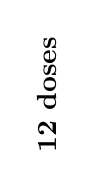
\begin{tikzpicture}
      \node[rotate=90] {\textbf{12 doses}};
    \end{tikzpicture}
  \end{subfigure}
  %
  \begin{subfigure}[c]{0.40\textwidth}
    \includegraphics[width=\textwidth]{figures/dose-response-d_diff-1-2-3-12doses-dil4-bowl-neg-controls-0.055.png}
  \end{subfigure}
  %
  \begin{subfigure}[c]{0.40\textwidth}
    \centering
    \includegraphics[width=\textwidth]{figures/dose-response-d_diff-1-2-3-12doses-dil4-bowl-neg-controls-0.085.png}
  \end{subfigure}

  \caption{Mean absolute difference between expected and obtained heights ($d_{\max}$) for dose-response curves using various numbers of doses, replicates, and \emph{bowl-shaped} plate-effect strengths. The 4PL sigmoid curves were fitted using compound data and 4 negative controls such that their mean was equal to the mean of the 20 negative controls on the plate. *** indicates $p\leq10^{-43}$.}
\end{figure*}

\begin{table}[H]
  \caption{%
    $d_{max}$ error overview for \emph{bowl-shaped} plate-effect strengths. Values are mean absolute differences in fitted $d_{max}$ across compounds. Best (lowest) value per row is \textbf{bolded}.
  }
  \label{tab:dr-overview-dmax-bowl-neg}
  \centering
  \input{tables/dr-overview-dmax-bowl-neg}
\end{table}


\clearpage
\subsubsection{Relative IC$_{50}$/EC$_{50}$ errors}

\begin{figure*}[!htbp]
  \centering
  \begin{subfigure}[c]{0.05\textwidth}
    ~
  \end{subfigure}
  %
  \begin{subfigure}[c]{0.40\textwidth}
    \centering
    ~~\textbf{Mild plate effects}
  \end{subfigure}
  %
  \begin{subfigure}[c]{0.40\textwidth}
    \centering
    ~~\textbf{Strong plate effects}
  \end{subfigure}

  \begin{subfigure}[c]{0.05\textwidth}
    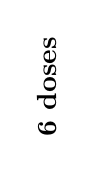
\begin{tikzpicture}
      \node[rotate=90] {\textbf{6 doses}};
    \end{tikzpicture}
  \end{subfigure}
  %
  \begin{subfigure}[c]{0.40\textwidth}
    \includegraphics[width=\textwidth]{figures/dose-response-relic50-1-2-3-6doses-dil18-bowl-neg-controls-0.055.png}
  \end{subfigure}
  %
  \begin{subfigure}[c]{0.40\textwidth}
    \centering
    \includegraphics[width=\textwidth]{figures/dose-response-relic50-1-2-3-6doses-dil18-bowl-neg-controls-0.085.png}
  \end{subfigure}

  \begin{subfigure}[c]{0.05\textwidth}
    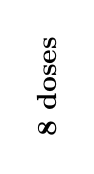
\begin{tikzpicture}
      \node[rotate=90] {\textbf{8 doses}};
    \end{tikzpicture}
  \end{subfigure}
  %
  \begin{subfigure}[c]{0.40\textwidth}
    \includegraphics[width=\textwidth]{figures/dose-response-relic50-1-2-3-8doses-dil8-bowl-neg-controls-0.055.png}
  \end{subfigure}
  %
  \begin{subfigure}[c]{0.40\textwidth}
    \centering
    \includegraphics[width=\textwidth]{figures/dose-response-relic50-1-2-3-8doses-dil8-bowl-neg-controls-0.085.png}
  \end{subfigure}

  \begin{subfigure}[c]{0.05\textwidth}
    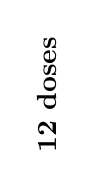
\begin{tikzpicture}
      \node[rotate=90] {\textbf{12 doses}};
    \end{tikzpicture}
  \end{subfigure}
  %
  \begin{subfigure}[c]{0.40\textwidth}
    \includegraphics[width=\textwidth]{figures/dose-response-relic50-1-2-3-12doses-dil4-bowl-neg-controls-0.055.png}
  \end{subfigure}
  %
  \begin{subfigure}[c]{0.40\textwidth}
    \centering
    \includegraphics[width=\textwidth]{figures/dose-response-relic50-1-2-3-12doses-dil4-bowl-neg-controls-0.085.png}
  \end{subfigure}

  \caption{Relative IC$_{50}$/EC$_{50}$ error for dose-response curves using various numbers of doses, replicates, and \emph{bowl-shaped} plate-effect strengths. *** indicates $p\leq10^{-43}$.}
\end{figure*}

\begin{table}[H]
  \caption{%
    Relative IC$_{50}$/EC$_{50}$ MSE overview for \emph{bowl-shaped} plate-effect strengths. Best (lowest) value per row is \textbf{bolded}.
  }
  \label{tab:dr-overview-rel-ic50-bowl-neg}
  \centering
  \input{tables/dr-overview-rel-ic50-bowl-neg}
\end{table}


\clearpage
\subsubsection{Absolute IC$_{50}$/EC$_{50}$ errors}

\begin{figure*}[!htbp]
  \centering
  \begin{subfigure}[c]{0.05\textwidth}
    ~
  \end{subfigure}
  %
  \begin{subfigure}[c]{0.40\textwidth}
    \centering
    ~~\textbf{Mild plate effects}
  \end{subfigure}
  %
  \begin{subfigure}[c]{0.40\textwidth}
    \centering
    ~~\textbf{Strong plate effects}
  \end{subfigure}

  \begin{subfigure}[c]{0.05\textwidth}
    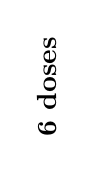
\begin{tikzpicture}
      \node[rotate=90] {\textbf{6 doses}};
    \end{tikzpicture}
  \end{subfigure}
  %
  \begin{subfigure}[c]{0.40\textwidth}
    \includegraphics[width=\textwidth]{figures/dose-response-absic50-1-2-3-6doses-dil18-bowl-neg-controls-0.055.png}
  \end{subfigure}
  %
  \begin{subfigure}[c]{0.40\textwidth}
    \centering
    \includegraphics[width=\textwidth]{figures/dose-response-absic50-1-2-3-6doses-dil18-bowl-neg-controls-0.085.png}
  \end{subfigure}

  \begin{subfigure}[c]{0.05\textwidth}
    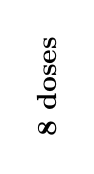
\begin{tikzpicture}
      \node[rotate=90] {\textbf{8 doses}};
    \end{tikzpicture}
  \end{subfigure}
  %
  \begin{subfigure}[c]{0.40\textwidth}
    \includegraphics[width=\textwidth]{figures/dose-response-absic50-1-2-3-8doses-dil8-bowl-neg-controls-0.055.png}
  \end{subfigure}
  %
  \begin{subfigure}[c]{0.40\textwidth}
    \centering
    \includegraphics[width=\textwidth]{figures/dose-response-absic50-1-2-3-8doses-dil8-bowl-neg-controls-0.085.png}
  \end{subfigure}

  \begin{subfigure}[c]{0.05\textwidth}
    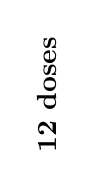
\begin{tikzpicture}
      \node[rotate=90] {\textbf{12 doses}};
    \end{tikzpicture}
  \end{subfigure}
  %
  \begin{subfigure}[c]{0.40\textwidth}
    \includegraphics[width=\textwidth]{figures/dose-response-absic50-1-2-3-12doses-dil4-bowl-neg-controls-0.055.png}
  \end{subfigure}
  %
  \begin{subfigure}[c]{0.40\textwidth}
    \centering
    \includegraphics[width=\textwidth]{figures/dose-response-absic50-1-2-3-12doses-dil4-bowl-neg-controls-0.085.png}
  \end{subfigure}

  \caption{Absolute IC$_{50}$/EC$_{50}$ error for dose-response curves using various numbers of doses, replicates, and \emph{bowl-shaped} plate-effect strengths. *** indicates $p\leq10^{-43}$.}
\end{figure*}

\begin{table}[H]
  \caption{%
    Absolute IC$_{50}$/EC$_{50}$ error overview for \emph{bowl-shaped} plate-effect strengths. Values are mean squared absolute IC$_{50}$/EC$_{50}$ estimation errors across compounds. Best (lowest) value per row is \textbf{bolded}.
  }
  \label{tab:dr-overview-abs-ic50-bowl-neg}
  \centering
  \input{tables/dr-overview-abs-ic50-bowl-neg}
\end{table}


\clearpage
\subsubsection{Residuals}

\begin{figure*}[!htbp]
  \centering
  \begin{subfigure}[c]{0.05\textwidth}
    ~
  \end{subfigure}
  %
  \begin{subfigure}[c]{0.40\textwidth}
    \centering
    ~~\textbf{Mild plate effects}
  \end{subfigure}
  %
  \begin{subfigure}[c]{0.40\textwidth}
    \centering
    ~~\textbf{Strong plate effects}
  \end{subfigure}

  \begin{subfigure}[c]{0.05\textwidth}
    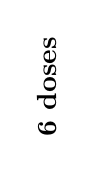
\begin{tikzpicture}
      \node[rotate=90] {\textbf{6 doses}};
    \end{tikzpicture}
  \end{subfigure}
  %
  \begin{subfigure}[c]{0.40\textwidth}
    \includegraphics[width=\textwidth]{figures/residuals-1-2-3-6doses-dil18-bowl-neg-controls-0.055.png}
  \end{subfigure}
  %
  \begin{subfigure}[c]{0.40\textwidth}
    \centering
    \includegraphics[width=\textwidth]{figures/residuals-1-2-3-6doses-dil18-bowl-neg-controls-0.085.png}
  \end{subfigure}

  \begin{subfigure}[c]{0.05\textwidth}
    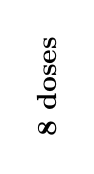
\begin{tikzpicture}
      \node[rotate=90] {\textbf{8 doses}};
    \end{tikzpicture}
  \end{subfigure}
  %
  \begin{subfigure}[c]{0.40\textwidth}
    \includegraphics[width=\textwidth]{figures/residuals-1-2-3-8doses-dil8-bowl-neg-controls-0.055.png}
  \end{subfigure}
  %
  \begin{subfigure}[c]{0.40\textwidth}
    \centering
    \includegraphics[width=\textwidth]{figures/residuals-1-2-3-8doses-dil8-bowl-neg-controls-0.085.png}
  \end{subfigure}

  \begin{subfigure}[c]{0.05\textwidth}
    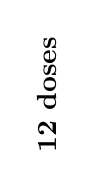
\begin{tikzpicture}
      \node[rotate=90] {\textbf{12 doses}};
    \end{tikzpicture}
  \end{subfigure}
  %
  \begin{subfigure}[c]{0.40\textwidth}
    \includegraphics[width=\textwidth]{figures/residuals-1-2-3-12doses-dil4-bowl-neg-controls-0.055.png}
  \end{subfigure}
  %
  \begin{subfigure}[c]{0.40\textwidth}
    \centering
    \includegraphics[width=\textwidth]{figures/residuals-1-2-3-12doses-dil4-bowl-neg-controls-0.085.png}
  \end{subfigure}

  \caption{Residuals (MSE between expected and obtained responses) for dose-response simulations using various numbers of doses, replicates, and \emph{bowl-shaped} plate-effect strengths. *** indicates $p\leq10^{-43}$.}
\end{figure*}

\begin{table}[H]
  \caption{%
    Residual MSE overview for \emph{bowl-shaped} plate-effect strengths. Best (lowest) value per row is \textbf{bolded}.
  }
  \label{tab:dr-overview-residuals-bowl-neg}
  \centering
  \input{tables/dr-overview-residuals-bowl-neg}
\end{table}


\clearpage
\subsubsection{Fraction of poor fits (low $R^2$)}

\begin{figure*}[!htbp]
  \centering
  \begin{subfigure}[c]{0.05\textwidth}
    ~
  \end{subfigure}
  %
  \begin{subfigure}[c]{0.40\textwidth}
    \centering
    ~~\textbf{Mild plate effects}
  \end{subfigure}
  %
  \begin{subfigure}[c]{0.40\textwidth}
    \centering
    ~~\textbf{Strong plate effects}
  \end{subfigure}

  \begin{subfigure}[c]{0.05\textwidth}
    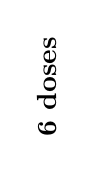
\begin{tikzpicture}
      \node[rotate=90] {\textbf{6 doses}};
    \end{tikzpicture}
  \end{subfigure}
  %
  \begin{subfigure}[c]{0.40\textwidth}
    \includegraphics[width=\textwidth]{figures/percentage-low-r2-curves-1-2-3-6doses-dil18-bowl-neg-controls-0.055.png}
  \end{subfigure}
  %
  \begin{subfigure}[c]{0.40\textwidth}
    \centering
    \includegraphics[width=\textwidth]{figures/percentage-low-r2-curves-1-2-3-6doses-dil18-bowl-neg-controls-0.085.png}
  \end{subfigure}

  \begin{subfigure}[c]{0.05\textwidth}
    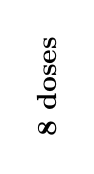
\begin{tikzpicture}
      \node[rotate=90] {\textbf{8 doses}};
    \end{tikzpicture}
  \end{subfigure}
  %
  \begin{subfigure}[c]{0.40\textwidth}
    \includegraphics[width=\textwidth]{figures/percentage-low-r2-curves-1-2-3-8doses-dil8-bowl-neg-controls-0.055.png}
  \end{subfigure}
  %
  \begin{subfigure}[c]{0.40\textwidth}
    \centering
    \includegraphics[width=\textwidth]{figures/percentage-low-r2-curves-1-2-3-8doses-dil8-bowl-neg-controls-0.085.png}
  \end{subfigure}

  \begin{subfigure}[c]{0.05\textwidth}
    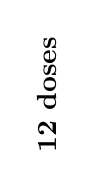
\begin{tikzpicture}
      \node[rotate=90] {\textbf{12 doses}};
    \end{tikzpicture}
  \end{subfigure}
  %
  \begin{subfigure}[c]{0.40\textwidth}
    \includegraphics[width=\textwidth]{figures/percentage-low-r2-curves-1-2-3-12doses-dil4-bowl-neg-controls-0.055.png}
  \end{subfigure}
  %
  \begin{subfigure}[c]{0.40\textwidth}
    \centering
    \includegraphics[width=\textwidth]{figures/percentage-low-r2-curves-1-2-3-12doses-dil4-bowl-neg-controls-0.085.png}
  \end{subfigure}

  \caption{Percentage of dose-response curves with low-quality ($R^2 < 80\%$) using various numbers of doses, replicates, and \emph{bowl-shaped} plate-effect strengths. The 4PL sigmoid curves were fitted using compound data and 4 negative controls such that their mean was equal to the mean of the 20 negative controls on the plate.}
\end{figure*}

\clearpage
\subsection{\emph{half-column} plate effects (column (half-plate))}


\subsubsection{$d_{\max}$ errors}

\begin{figure*}[!htbp]
  \centering
  \begin{subfigure}[c]{0.05\textwidth}
    ~
  \end{subfigure}
  %
  \begin{subfigure}[c]{0.40\textwidth}
    \centering
    ~~\textbf{Mild plate effects}
  \end{subfigure}
  %
  \begin{subfigure}[c]{0.40\textwidth}
    \centering
    ~~\textbf{Strong plate effects}
  \end{subfigure}

  \begin{subfigure}[c]{0.05\textwidth}
    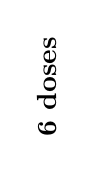
\begin{tikzpicture}
      \node[rotate=90] {\textbf{6 doses}};
    \end{tikzpicture}
  \end{subfigure}
  %
  \begin{subfigure}[c]{0.40\textwidth}
    \includegraphics[width=\textwidth]{figures/dose-response-d_diff-1-2-3-6doses-dil18-half-columns-neg-controls-0.2.png}
  \end{subfigure}
  %
  \begin{subfigure}[c]{0.40\textwidth}
    \centering
    \includegraphics[width=\textwidth]{figures/dose-response-d_diff-1-2-3-6doses-dil18-half-columns-neg-controls-0.4.png}
  \end{subfigure}

  \begin{subfigure}[c]{0.05\textwidth}
    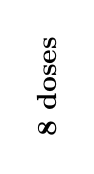
\begin{tikzpicture}
      \node[rotate=90] {\textbf{8 doses}};
    \end{tikzpicture}
  \end{subfigure}
  %
  \begin{subfigure}[c]{0.40\textwidth}
    \includegraphics[width=\textwidth]{figures/dose-response-d_diff-1-2-3-8doses-dil8-half-columns-neg-controls-0.2.png}
  \end{subfigure}
  %
  \begin{subfigure}[c]{0.40\textwidth}
    \centering
    \includegraphics[width=\textwidth]{figures/dose-response-d_diff-1-2-3-8doses-dil8-half-columns-neg-controls-0.4.png}
  \end{subfigure}

  \begin{subfigure}[c]{0.05\textwidth}
    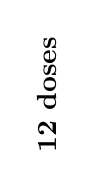
\begin{tikzpicture}
      \node[rotate=90] {\textbf{12 doses}};
    \end{tikzpicture}
  \end{subfigure}
  %
  \begin{subfigure}[c]{0.40\textwidth}
    \includegraphics[width=\textwidth]{figures/dose-response-d_diff-1-2-3-12doses-dil4-half-columns-neg-controls-0.2.png}
  \end{subfigure}
  %
  \begin{subfigure}[c]{0.40\textwidth}
    \centering
    \includegraphics[width=\textwidth]{figures/dose-response-d_diff-1-2-3-12doses-dil4-half-columns-neg-controls-0.4.png}
  \end{subfigure}

  \caption{Mean absolute difference between expected and obtained heights ($d_{\max}$) for dose-response curves using various numbers of doses, replicates, and \emph{half-column} plate-effect strengths. The 4PL sigmoid curves were fitted using compound data and 4 negative controls such that their mean was equal to the mean of the 20 negative controls on the plate. *** indicates $p\leq10^{-43}$.}
\end{figure*}

\begin{table}[H]
  \caption{%
    $d_{max}$ error overview for \emph{half-column} plate-effect strengths. Values are mean absolute differences in fitted $d_{max}$ across compounds. Best (lowest) value per row is \textbf{bolded}.
  }
  \label{tab:dr-overview-dmax-column}
  \centering
  \input{tables/dr-overview-dmax-column}
\end{table}


\clearpage
\subsubsection{Relative IC$_{50}$/EC$_{50}$ errors}

\begin{figure*}[!htbp]
  \centering
  \begin{subfigure}[c]{0.05\textwidth}
    ~
  \end{subfigure}
  %
  \begin{subfigure}[c]{0.40\textwidth}
    \centering
    ~~\textbf{Mild plate effects}
  \end{subfigure}
  %
  \begin{subfigure}[c]{0.40\textwidth}
    \centering
    ~~\textbf{Strong plate effects}
  \end{subfigure}

  \begin{subfigure}[c]{0.05\textwidth}
    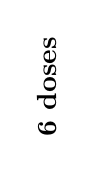
\begin{tikzpicture}
      \node[rotate=90] {\textbf{6 doses}};
    \end{tikzpicture}
  \end{subfigure}
  %
  \begin{subfigure}[c]{0.40\textwidth}
    \includegraphics[width=\textwidth]{figures/dose-response-relic50-1-2-3-6doses-dil18-half-columns-neg-controls-0.2.png}
  \end{subfigure}
  %
  \begin{subfigure}[c]{0.40\textwidth}
    \centering
    \includegraphics[width=\textwidth]{figures/dose-response-relic50-1-2-3-6doses-dil18-half-columns-neg-controls-0.4.png}
  \end{subfigure}

  \begin{subfigure}[c]{0.05\textwidth}
    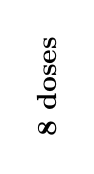
\begin{tikzpicture}
      \node[rotate=90] {\textbf{8 doses}};
    \end{tikzpicture}
  \end{subfigure}
  %
  \begin{subfigure}[c]{0.40\textwidth}
    \includegraphics[width=\textwidth]{figures/dose-response-relic50-1-2-3-8doses-dil8-half-columns-neg-controls-0.2.png}
  \end{subfigure}
  %
  \begin{subfigure}[c]{0.40\textwidth}
    \centering
    \includegraphics[width=\textwidth]{figures/dose-response-relic50-1-2-3-8doses-dil8-half-columns-neg-controls-0.4.png}
  \end{subfigure}

  \begin{subfigure}[c]{0.05\textwidth}
    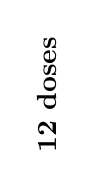
\begin{tikzpicture}
      \node[rotate=90] {\textbf{12 doses}};
    \end{tikzpicture}
  \end{subfigure}
  %
  \begin{subfigure}[c]{0.40\textwidth}
    \includegraphics[width=\textwidth]{figures/dose-response-relic50-1-2-3-12doses-dil4-half-columns-neg-controls-0.2.png}
  \end{subfigure}
  %
  \begin{subfigure}[c]{0.40\textwidth}
    \centering
    \includegraphics[width=\textwidth]{figures/dose-response-relic50-1-2-3-12doses-dil4-half-columns-neg-controls-0.4.png}
  \end{subfigure}

  \caption{Relative IC$_{50}$/EC$_{50}$ error for dose-response curves using various numbers of doses, replicates, and \emph{half-column} plate-effect strengths. *** indicates $p\leq10^{-43}$.}
\end{figure*}

\begin{table}[H]
  \caption{%
    Relative IC$_{50}$/EC$_{50}$ MSE overview for \emph{half-column} plate-effect strengths. Best (lowest) value per row is \textbf{bolded}.
  }
  \label{tab:dr-overview-rel-ic50-column}
  \centering
  \input{tables/dr-overview-rel-ic50-column}
\end{table}


\clearpage
\subsubsection{Absolute IC$_{50}$/EC$_{50}$ errors}

\begin{figure*}[!htbp]
  \centering
  \begin{subfigure}[c]{0.05\textwidth}
    ~
  \end{subfigure}
  %
  \begin{subfigure}[c]{0.40\textwidth}
    \centering
    ~~\textbf{Mild plate effects}
  \end{subfigure}
  %
  \begin{subfigure}[c]{0.40\textwidth}
    \centering
    ~~\textbf{Strong plate effects}
  \end{subfigure}

  \begin{subfigure}[c]{0.05\textwidth}
    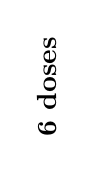
\begin{tikzpicture}
      \node[rotate=90] {\textbf{6 doses}};
    \end{tikzpicture}
  \end{subfigure}
  %
  \begin{subfigure}[c]{0.40\textwidth}
    \includegraphics[width=\textwidth]{figures/dose-response-absic50-1-2-3-6doses-dil18-half-columns-neg-controls-0.2.png}
  \end{subfigure}
  %
  \begin{subfigure}[c]{0.40\textwidth}
    \centering
    \includegraphics[width=\textwidth]{figures/dose-response-absic50-1-2-3-6doses-dil18-half-columns-neg-controls-0.4.png}
  \end{subfigure}

  \begin{subfigure}[c]{0.05\textwidth}
    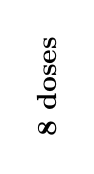
\begin{tikzpicture}
      \node[rotate=90] {\textbf{8 doses}};
    \end{tikzpicture}
  \end{subfigure}
  %
  \begin{subfigure}[c]{0.40\textwidth}
    \includegraphics[width=\textwidth]{figures/dose-response-absic50-1-2-3-8doses-dil8-half-columns-neg-controls-0.2.png}
  \end{subfigure}
  %
  \begin{subfigure}[c]{0.40\textwidth}
    \centering
    \includegraphics[width=\textwidth]{figures/dose-response-absic50-1-2-3-8doses-dil8-half-columns-neg-controls-0.4.png}
  \end{subfigure}

  \begin{subfigure}[c]{0.05\textwidth}
    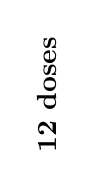
\begin{tikzpicture}
      \node[rotate=90] {\textbf{12 doses}};
    \end{tikzpicture}
  \end{subfigure}
  %
  \begin{subfigure}[c]{0.40\textwidth}
    \includegraphics[width=\textwidth]{figures/dose-response-absic50-1-2-3-12doses-dil4-half-columns-neg-controls-0.2.png}
  \end{subfigure}
  %
  \begin{subfigure}[c]{0.40\textwidth}
    \centering
    \includegraphics[width=\textwidth]{figures/dose-response-absic50-1-2-3-12doses-dil4-half-columns-neg-controls-0.4.png}
  \end{subfigure}

  \caption{Absolute IC$_{50}$/EC$_{50}$ error for dose-response curves using various numbers of doses, replicates, and \emph{half-column} plate-effect strengths. *** indicates $p\leq10^{-43}$.}
\end{figure*}

\begin{table}[H]
  \caption{%
    Absolute IC$_{50}$/EC$_{50}$ error overview for \emph{half-column} plate-effect strengths. Values are mean squared absolute IC$_{50}$/EC$_{50}$ estimation errors across compounds. Best (lowest) value per row is \textbf{bolded}.
  }
  \label{tab:dr-overview-abs-ic50-column}
  \centering
  \input{tables/dr-overview-abs-ic50-column}
\end{table}


\clearpage
\subsubsection{Residuals}

\begin{figure*}[!htbp]
  \centering
  \begin{subfigure}[c]{0.05\textwidth}
    ~
  \end{subfigure}
  %
  \begin{subfigure}[c]{0.40\textwidth}
    \centering
    ~~\textbf{Mild plate effects}
  \end{subfigure}
  %
  \begin{subfigure}[c]{0.40\textwidth}
    \centering
    ~~\textbf{Strong plate effects}
  \end{subfigure}

  \begin{subfigure}[c]{0.05\textwidth}
    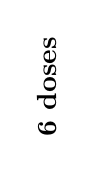
\begin{tikzpicture}
      \node[rotate=90] {\textbf{6 doses}};
    \end{tikzpicture}
  \end{subfigure}
  %
  \begin{subfigure}[c]{0.40\textwidth}
    \includegraphics[width=\textwidth]{figures/residuals-1-2-3-6doses-dil18-half-columns-neg-controls-0.2.png}
  \end{subfigure}
  %
  \begin{subfigure}[c]{0.40\textwidth}
    \centering
    \includegraphics[width=\textwidth]{figures/residuals-1-2-3-6doses-dil18-half-columns-neg-controls-0.4.png}
  \end{subfigure}

  \begin{subfigure}[c]{0.05\textwidth}
    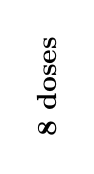
\begin{tikzpicture}
      \node[rotate=90] {\textbf{8 doses}};
    \end{tikzpicture}
  \end{subfigure}
  %
  \begin{subfigure}[c]{0.40\textwidth}
    \includegraphics[width=\textwidth]{figures/residuals-1-2-3-8doses-dil8-half-columns-neg-controls-0.2.png}
  \end{subfigure}
  %
  \begin{subfigure}[c]{0.40\textwidth}
    \centering
    \includegraphics[width=\textwidth]{figures/residuals-1-2-3-8doses-dil8-half-columns-neg-controls-0.4.png}
  \end{subfigure}

  \begin{subfigure}[c]{0.05\textwidth}
    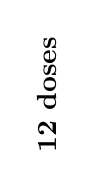
\begin{tikzpicture}
      \node[rotate=90] {\textbf{12 doses}};
    \end{tikzpicture}
  \end{subfigure}
  %
  \begin{subfigure}[c]{0.40\textwidth}
    \includegraphics[width=\textwidth]{figures/residuals-1-2-3-12doses-dil4-half-columns-neg-controls-0.2.png}
  \end{subfigure}
  %
  \begin{subfigure}[c]{0.40\textwidth}
    \centering
    \includegraphics[width=\textwidth]{figures/residuals-1-2-3-12doses-dil4-half-columns-neg-controls-0.4.png}
  \end{subfigure}

  \caption{Residuals (MSE between expected and obtained responses) for dose-response simulations using various numbers of doses, replicates, and \emph{half-column} plate-effect strengths. *** indicates $p\leq10^{-43}$.}
\end{figure*}

\begin{table}[H]
  \caption{%
    Residual MSE overview for \emph{half-column} plate-effect strengths. Best (lowest) value per row is \textbf{bolded}.
  }
  \label{tab:dr-overview-residuals-column}
  \centering
  \input{tables/dr-overview-residuals-column}
\end{table}


\clearpage
\subsection{\emph{row-gradient} plate effects (row gradient (top-to-bottom))}


\subsubsection{$d_{\max}$ errors}

\begin{figure*}[!htbp]
  \centering
  \begin{subfigure}[c]{0.05\textwidth}
    ~
  \end{subfigure}
  %
  \begin{subfigure}[c]{0.40\textwidth}
    \centering
    ~~\textbf{Mild plate effects}
  \end{subfigure}
  %
  \begin{subfigure}[c]{0.40\textwidth}
    \centering
    ~~\textbf{Strong plate effects}
  \end{subfigure}

  \begin{subfigure}[c]{0.05\textwidth}
    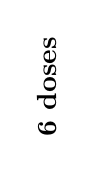
\begin{tikzpicture}
      \node[rotate=90] {\textbf{6 doses}};
    \end{tikzpicture}
  \end{subfigure}
  %
  \begin{subfigure}[c]{0.40\textwidth}
    \includegraphics[width=\textwidth]{figures/dose-response-d_diff-1-2-3-6doses-dil18-row-gradient-0.006.png}
  \end{subfigure}
  %
  \begin{subfigure}[c]{0.40\textwidth}
    \centering
    \includegraphics[width=\textwidth]{figures/dose-response-d_diff-1-2-3-6doses-dil18-row-gradient-0.012.png}
  \end{subfigure}

  \begin{subfigure}[c]{0.05\textwidth}
    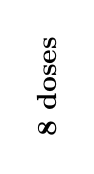
\begin{tikzpicture}
      \node[rotate=90] {\textbf{8 doses}};
    \end{tikzpicture}
  \end{subfigure}
  %
  \begin{subfigure}[c]{0.40\textwidth}
    \includegraphics[width=\textwidth]{figures/dose-response-d_diff-1-2-3-8doses-dil8-row-gradient-0.006.png}
  \end{subfigure}
  %
  \begin{subfigure}[c]{0.40\textwidth}
    \centering
    \includegraphics[width=\textwidth]{figures/dose-response-d_diff-1-2-3-8doses-dil8-row-gradient-0.012.png}
  \end{subfigure}

  \begin{subfigure}[c]{0.05\textwidth}
    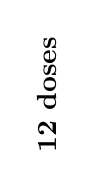
\begin{tikzpicture}
      \node[rotate=90] {\textbf{12 doses}};
    \end{tikzpicture}
  \end{subfigure}
  %
  \begin{subfigure}[c]{0.40\textwidth}
    \includegraphics[width=\textwidth]{figures/dose-response-d_diff-1-2-3-12doses-dil4-row-gradient-0.006.png}
  \end{subfigure}
  %
  \begin{subfigure}[c]{0.40\textwidth}
    \centering
    \includegraphics[width=\textwidth]{figures/dose-response-d_diff-1-2-3-12doses-dil4-row-gradient-0.012.png}
  \end{subfigure}

  \caption{Mean absolute difference between expected and obtained heights ($d_{\max}$) for dose-response curves using various numbers of doses, replicates, and \emph{row-gradient} plate-effect strengths. The 4PL sigmoid curves were fitted using compound data and 4 negative controls such that their mean was equal to the mean of the 20 negative controls on the plate. *** indicates $p\leq10^{-43}$.}
\end{figure*}

\begin{table}[H]
  \caption{%
    $d_{max}$ error overview for \emph{row-gradient} plate-effect strengths. Values are mean absolute differences in fitted $d_{max}$ across compounds. Best (lowest) value per row is \textbf{bolded}.
  }
  \label{tab:dr-overview-dmax-row-gradient}
  \centering
  \input{tables/dr-overview-dmax-row-gradient}
\end{table}


\clearpage
\subsubsection{Relative IC$_{50}$/EC$_{50}$ errors}

\begin{figure*}[!htbp]
  \centering
  \begin{subfigure}[c]{0.05\textwidth}
    ~
  \end{subfigure}
  %
  \begin{subfigure}[c]{0.40\textwidth}
    \centering
    ~~\textbf{Mild plate effects}
  \end{subfigure}
  %
  \begin{subfigure}[c]{0.40\textwidth}
    \centering
    ~~\textbf{Strong plate effects}
  \end{subfigure}

  \begin{subfigure}[c]{0.05\textwidth}
    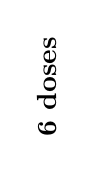
\begin{tikzpicture}
      \node[rotate=90] {\textbf{6 doses}};
    \end{tikzpicture}
  \end{subfigure}
  %
  \begin{subfigure}[c]{0.40\textwidth}
    \includegraphics[width=\textwidth]{figures/dose-response-relic50-1-2-3-6doses-dil18-row-gradient-0.006.png}
  \end{subfigure}
  %
  \begin{subfigure}[c]{0.40\textwidth}
    \centering
    \includegraphics[width=\textwidth]{figures/dose-response-relic50-1-2-3-6doses-dil18-row-gradient-0.012.png}
  \end{subfigure}

  \begin{subfigure}[c]{0.05\textwidth}
    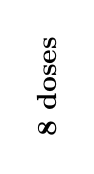
\begin{tikzpicture}
      \node[rotate=90] {\textbf{8 doses}};
    \end{tikzpicture}
  \end{subfigure}
  %
  \begin{subfigure}[c]{0.40\textwidth}
    \includegraphics[width=\textwidth]{figures/dose-response-relic50-1-2-3-8doses-dil8-row-gradient-0.006.png}
  \end{subfigure}
  %
  \begin{subfigure}[c]{0.40\textwidth}
    \centering
    \includegraphics[width=\textwidth]{figures/dose-response-relic50-1-2-3-8doses-dil8-row-gradient-0.012.png}
  \end{subfigure}

  \begin{subfigure}[c]{0.05\textwidth}
    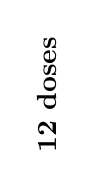
\begin{tikzpicture}
      \node[rotate=90] {\textbf{12 doses}};
    \end{tikzpicture}
  \end{subfigure}
  %
  \begin{subfigure}[c]{0.40\textwidth}
    \includegraphics[width=\textwidth]{figures/dose-response-relic50-1-2-3-12doses-dil4-row-gradient-0.006.png}
  \end{subfigure}
  %
  \begin{subfigure}[c]{0.40\textwidth}
    \centering
    \includegraphics[width=\textwidth]{figures/dose-response-relic50-1-2-3-12doses-dil4-row-gradient-0.012.png}
  \end{subfigure}

  \caption{Relative IC$_{50}$/EC$_{50}$ error for dose-response curves using various numbers of doses, replicates, and \emph{row-gradient} plate-effect strengths. *** indicates $p\leq10^{-43}$.}
\end{figure*}

\begin{table}[H]
  \caption{%
    Relative IC$_{50}$/EC$_{50}$ MSE overview for \emph{row-gradient} plate-effect strengths. Best (lowest) value per row is \textbf{bolded}.
  }
  \label{tab:dr-overview-rel-ic50-row-gradient}
  \centering
  \input{tables/dr-overview-rel-ic50-row-gradient}
\end{table}


\clearpage
\subsubsection{Absolute IC$_{50}$/EC$_{50}$ errors}

\begin{figure*}[!htbp]
  \centering
  \begin{subfigure}[c]{0.05\textwidth}
    ~
  \end{subfigure}
  %
  \begin{subfigure}[c]{0.40\textwidth}
    \centering
    ~~\textbf{Mild plate effects}
  \end{subfigure}
  %
  \begin{subfigure}[c]{0.40\textwidth}
    \centering
    ~~\textbf{Strong plate effects}
  \end{subfigure}

  \begin{subfigure}[c]{0.05\textwidth}
    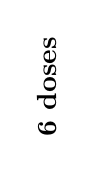
\begin{tikzpicture}
      \node[rotate=90] {\textbf{6 doses}};
    \end{tikzpicture}
  \end{subfigure}
  %
  \begin{subfigure}[c]{0.40\textwidth}
    \includegraphics[width=\textwidth]{figures/dose-response-absic50-1-2-3-6doses-dil18-row-gradient-0.006.png}
  \end{subfigure}
  %
  \begin{subfigure}[c]{0.40\textwidth}
    \centering
    \includegraphics[width=\textwidth]{figures/dose-response-absic50-1-2-3-6doses-dil18-row-gradient-0.012.png}
  \end{subfigure}

  \begin{subfigure}[c]{0.05\textwidth}
    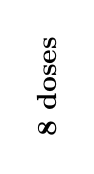
\begin{tikzpicture}
      \node[rotate=90] {\textbf{8 doses}};
    \end{tikzpicture}
  \end{subfigure}
  %
  \begin{subfigure}[c]{0.40\textwidth}
    \includegraphics[width=\textwidth]{figures/dose-response-absic50-1-2-3-8doses-dil8-row-gradient-0.006.png}
  \end{subfigure}
  %
  \begin{subfigure}[c]{0.40\textwidth}
    \centering
    \includegraphics[width=\textwidth]{figures/dose-response-absic50-1-2-3-8doses-dil8-row-gradient-0.012.png}
  \end{subfigure}

  \begin{subfigure}[c]{0.05\textwidth}
    \begin{tikzpicture}
      \node[rotate=90] {\textbf{12 doses}};
    \end{tikzpicture}
  \end{subfigure}
  %
  \begin{subfigure}[c]{0.40\textwidth}
    \includegraphics[width=\textwidth]{figures/dose-response-absic50-1-2-3-12doses-dil4-row-gradient-0.006.png}
  \end{subfigure}
  %
  \begin{subfigure}[c]{0.40\textwidth}
    \centering
    \includegraphics[width=\textwidth]{figures/dose-response-absic50-1-2-3-12doses-dil4-row-gradient-0.012.png}
  \end{subfigure}

  \caption{Absolute IC$_{50}$/EC$_{50}$ error for dose-response curves using various numbers of doses, replicates, and \emph{row-gradient} plate-effect strengths. *** indicates $p\leq10^{-43}$.}
\end{figure*}

\begin{table}[H]
  \caption{%
    Absolute IC$_{50}$/EC$_{50}$ error overview for \emph{row-gradient} plate-effect strengths. Values are mean squared absolute IC$_{50}$/EC$_{50}$ estimation errors across compounds. Best (lowest) value per row is \textbf{bolded}.
  }
  \label{tab:dr-overview-abs-ic50-row-gradient}
  \centering
  \input{tables/dr-overview-abs-ic50-row-gradient}
\end{table}


\clearpage
\subsubsection{Residuals}

\begin{figure*}[!htbp]
  \centering
  \begin{subfigure}[c]{0.05\textwidth}
    ~
  \end{subfigure}
  %
  \begin{subfigure}[c]{0.40\textwidth}
    \centering
    ~~\textbf{Mild plate effects}
  \end{subfigure}
  %
  \begin{subfigure}[c]{0.40\textwidth}
    \centering
    ~~\textbf{Strong plate effects}
  \end{subfigure}

  \begin{subfigure}[c]{0.05\textwidth}
    \begin{tikzpicture}
      \node[rotate=90] {\textbf{6 doses}};
    \end{tikzpicture}
  \end{subfigure}
  %
  \begin{subfigure}[c]{0.40\textwidth}
    \includegraphics[width=\textwidth]{figures/residuals-1-2-3-6doses-dil18-row-gradient-0.006.png}
  \end{subfigure}
  %
  \begin{subfigure}[c]{0.40\textwidth}
    \centering
    \includegraphics[width=\textwidth]{figures/residuals-1-2-3-6doses-dil18-row-gradient-0.012.png}
  \end{subfigure}

  \begin{subfigure}[c]{0.05\textwidth}
    \begin{tikzpicture}
      \node[rotate=90] {\textbf{8 doses}};
    \end{tikzpicture}
  \end{subfigure}
  %
  \begin{subfigure}[c]{0.40\textwidth}
    \includegraphics[width=\textwidth]{figures/residuals-1-2-3-8doses-dil8-row-gradient-0.006.png}
  \end{subfigure}
  %
  \begin{subfigure}[c]{0.40\textwidth}
    \centering
    \includegraphics[width=\textwidth]{figures/residuals-1-2-3-8doses-dil8-row-gradient-0.012.png}
  \end{subfigure}

  \begin{subfigure}[c]{0.05\textwidth}
    \begin{tikzpicture}
      \node[rotate=90] {\textbf{12 doses}};
    \end{tikzpicture}
  \end{subfigure}
  %
  \begin{subfigure}[c]{0.40\textwidth}
    \includegraphics[width=\textwidth]{figures/residuals-1-2-3-12doses-dil4-row-gradient-0.006.png}
  \end{subfigure}
  %
  \begin{subfigure}[c]{0.40\textwidth}
    \centering
    \includegraphics[width=\textwidth]{figures/residuals-1-2-3-12doses-dil4-row-gradient-0.012.png}
  \end{subfigure}

  \caption{Residuals (MSE between expected and obtained responses) for dose-response simulations using various numbers of doses, replicates, and \emph{row-gradient} plate-effect strengths. *** indicates $p\leq10^{-43}$.}
\end{figure*}

\begin{table}[H]
  \caption{%
    Residual MSE overview for \emph{row-gradient} plate-effect strengths. Best (lowest) value per row is \textbf{bolded}.
  }
  \label{tab:dr-overview-residuals-row-gradient}
  \centering
  \input{tables/dr-overview-residuals-row-gradient}
\end{table}


\clearpage
\subsubsection{Fraction of poor fits (low $R^2$)}

\begin{figure*}[!htbp]
  \centering
  \begin{subfigure}[c]{0.05\textwidth}
    ~
  \end{subfigure}
  %
  \begin{subfigure}[c]{0.40\textwidth}
    \centering
    ~~\textbf{Mild plate effects}
  \end{subfigure}
  %
  \begin{subfigure}[c]{0.40\textwidth}
    \centering
    ~~\textbf{Strong plate effects}
  \end{subfigure}

  \begin{subfigure}[c]{0.05\textwidth}
    \begin{tikzpicture}
      \node[rotate=90] {\textbf{6 doses}};
    \end{tikzpicture}
  \end{subfigure}
  %
  \begin{subfigure}[c]{0.40\textwidth}
    \includegraphics[width=\textwidth]{figures/percentage-low-r2-curves-1-2-3-6doses-dil18-row-gradient-0.006.png}
  \end{subfigure}
  %
  \begin{subfigure}[c]{0.40\textwidth}
    \centering
    \includegraphics[width=\textwidth]{figures/percentage-low-r2-curves-1-2-3-6doses-dil18-row-gradient-0.012.png}
  \end{subfigure}

  \begin{subfigure}[c]{0.05\textwidth}
    \begin{tikzpicture}
      \node[rotate=90] {\textbf{8 doses}};
    \end{tikzpicture}
  \end{subfigure}
  %
  \begin{subfigure}[c]{0.40\textwidth}
    \includegraphics[width=\textwidth]{figures/percentage-low-r2-curves-1-2-3-8doses-dil8-row-gradient-0.006.png}
  \end{subfigure}
  %
  \begin{subfigure}[c]{0.40\textwidth}
    \centering
    \includegraphics[width=\textwidth]{figures/percentage-low-r2-curves-1-2-3-8doses-dil8-row-gradient-0.012.png}
  \end{subfigure}

  \begin{subfigure}[c]{0.05\textwidth}
    \begin{tikzpicture}
      \node[rotate=90] {\textbf{12 doses}};
    \end{tikzpicture}
  \end{subfigure}
  %
  \begin{subfigure}[c]{0.40\textwidth}
    \includegraphics[width=\textwidth]{figures/percentage-low-r2-curves-1-2-3-12doses-dil4-row-gradient-0.006.png}
  \end{subfigure}
  %
  \begin{subfigure}[c]{0.40\textwidth}
    \centering
    \includegraphics[width=\textwidth]{figures/percentage-low-r2-curves-1-2-3-12doses-dil4-row-gradient-0.012.png}
  \end{subfigure}

  \caption{Percentage of dose-response curves with low-quality ($R^2 < 80\%$) using various numbers of doses, replicates, and \emph{row-gradient} plate-effect strengths. The 4PL sigmoid curves were fitted using compound data and 4 negative controls such that their mean was equal to the mean of the 20 negative controls on the plate.}
\end{figure*}

\clearpage
\subsection{\emph{striped-row} plate effects (row stripe (even rows elevated))}


\subsubsection{$d_{\max}$ errors}

\begin{figure*}[!htbp]
  \centering
  \begin{subfigure}[c]{0.05\textwidth}
    ~
  \end{subfigure}
  %
  \begin{subfigure}[c]{0.40\textwidth}
    \centering
    ~~\textbf{Mild plate effects}
  \end{subfigure}
  %
  \begin{subfigure}[c]{0.40\textwidth}
    \centering
    ~~\textbf{Strong plate effects}
  \end{subfigure}

  \begin{subfigure}[c]{0.05\textwidth}
    \begin{tikzpicture}
      \node[rotate=90] {\textbf{6 doses}};
    \end{tikzpicture}
  \end{subfigure}
  %
  \begin{subfigure}[c]{0.40\textwidth}
    \includegraphics[width=\textwidth]{figures/dose-response-d_diff-1-2-3-6doses-dil18-striped-row-even-0.05.png}
  \end{subfigure}
  %
  \begin{subfigure}[c]{0.40\textwidth}
    \centering
    \includegraphics[width=\textwidth]{figures/dose-response-d_diff-1-2-3-6doses-dil18-striped-row-even-0.1.png}
  \end{subfigure}

  \begin{subfigure}[c]{0.05\textwidth}
    \begin{tikzpicture}
      \node[rotate=90] {\textbf{8 doses}};
    \end{tikzpicture}
  \end{subfigure}
  %
  \begin{subfigure}[c]{0.40\textwidth}
    \includegraphics[width=\textwidth]{figures/dose-response-d_diff-1-2-3-8doses-dil8-striped-row-even-0.05.png}
  \end{subfigure}
  %
  \begin{subfigure}[c]{0.40\textwidth}
    \centering
    \includegraphics[width=\textwidth]{figures/dose-response-d_diff-1-2-3-8doses-dil8-striped-row-even-0.1.png}
  \end{subfigure}

  \begin{subfigure}[c]{0.05\textwidth}
    \begin{tikzpicture}
      \node[rotate=90] {\textbf{12 doses}};
    \end{tikzpicture}
  \end{subfigure}
  %
  \begin{subfigure}[c]{0.40\textwidth}
    \includegraphics[width=\textwidth]{figures/dose-response-d_diff-1-2-3-12doses-dil4-striped-row-even-0.05.png}
  \end{subfigure}
  %
  \begin{subfigure}[c]{0.40\textwidth}
    \centering
    \includegraphics[width=\textwidth]{figures/dose-response-d_diff-1-2-3-12doses-dil4-striped-row-even-0.1.png}
  \end{subfigure}

  \caption{Mean absolute difference between expected and obtained heights ($d_{\max}$) for dose-response curves using various numbers of doses, replicates, and \emph{striped-row} plate-effect strengths. The 4PL sigmoid curves were fitted using compound data and 4 negative controls such that their mean was equal to the mean of the 20 negative controls on the plate. *** indicates $p\leq10^{-43}$.}
\end{figure*}

\begin{table}[H]
  \caption{%
    $d_{max}$ error overview for \emph{striped-row} plate-effect strengths. Values are mean absolute differences in fitted $d_{max}$ across compounds. Best (lowest) value per row is \textbf{bolded}.
  }
  \label{tab:dr-overview-dmax-striped-row-even}
  \centering
  \input{tables/dr-overview-dmax-striped-row-even}
\end{table}


\clearpage
\subsubsection{Relative IC$_{50}$/EC$_{50}$ errors}

\begin{figure*}[!htbp]
  \centering
  \begin{subfigure}[c]{0.05\textwidth}
    ~
  \end{subfigure}
  %
  \begin{subfigure}[c]{0.40\textwidth}
    \centering
    ~~\textbf{Mild plate effects}
  \end{subfigure}
  %
  \begin{subfigure}[c]{0.40\textwidth}
    \centering
    ~~\textbf{Strong plate effects}
  \end{subfigure}

  \begin{subfigure}[c]{0.05\textwidth}
    \begin{tikzpicture}
      \node[rotate=90] {\textbf{6 doses}};
    \end{tikzpicture}
  \end{subfigure}
  %
  \begin{subfigure}[c]{0.40\textwidth}
    \includegraphics[width=\textwidth]{figures/dose-response-relic50-1-2-3-6doses-dil18-striped-row-even-0.05.png}
  \end{subfigure}
  %
  \begin{subfigure}[c]{0.40\textwidth}
    \centering
    \includegraphics[width=\textwidth]{figures/dose-response-relic50-1-2-3-6doses-dil18-striped-row-even-0.1.png}
  \end{subfigure}

  \begin{subfigure}[c]{0.05\textwidth}
    \begin{tikzpicture}
      \node[rotate=90] {\textbf{8 doses}};
    \end{tikzpicture}
  \end{subfigure}
  %
  \begin{subfigure}[c]{0.40\textwidth}
    \includegraphics[width=\textwidth]{figures/dose-response-relic50-1-2-3-8doses-dil8-striped-row-even-0.05.png}
  \end{subfigure}
  %
  \begin{subfigure}[c]{0.40\textwidth}
    \centering
    \includegraphics[width=\textwidth]{figures/dose-response-relic50-1-2-3-8doses-dil8-striped-row-even-0.1.png}
  \end{subfigure}

  \begin{subfigure}[c]{0.05\textwidth}
    \begin{tikzpicture}
      \node[rotate=90] {\textbf{12 doses}};
    \end{tikzpicture}
  \end{subfigure}
  %
  \begin{subfigure}[c]{0.40\textwidth}
    \includegraphics[width=\textwidth]{figures/dose-response-relic50-1-2-3-12doses-dil4-striped-row-even-0.05.png}
  \end{subfigure}
  %
  \begin{subfigure}[c]{0.40\textwidth}
    \centering
    \includegraphics[width=\textwidth]{figures/dose-response-relic50-1-2-3-12doses-dil4-striped-row-even-0.1.png}
  \end{subfigure}

  \caption{Relative IC$_{50}$/EC$_{50}$ error for dose-response curves using various numbers of doses, replicates, and \emph{striped-row} plate-effect strengths. *** indicates $p\leq10^{-43}$.}
\end{figure*}

\begin{table}[H]
  \caption{%
    Relative IC$_{50}$/EC$_{50}$ MSE overview for \emph{striped-row} plate-effect strengths. Best (lowest) value per row is \textbf{bolded}.
  }
  \label{tab:dr-overview-rel-ic50-striped-row-even}
  \centering
  \input{tables/dr-overview-rel-ic50-striped-row-even}
\end{table}


\clearpage
\subsubsection{Absolute IC$_{50}$/EC$_{50}$ errors}

\begin{figure*}[!htbp]
  \centering
  \begin{subfigure}[c]{0.05\textwidth}
    ~
  \end{subfigure}
  %
  \begin{subfigure}[c]{0.40\textwidth}
    \centering
    ~~\textbf{Mild plate effects}
  \end{subfigure}
  %
  \begin{subfigure}[c]{0.40\textwidth}
    \centering
    ~~\textbf{Strong plate effects}
  \end{subfigure}

  \begin{subfigure}[c]{0.05\textwidth}
    \begin{tikzpicture}
      \node[rotate=90] {\textbf{6 doses}};
    \end{tikzpicture}
  \end{subfigure}
  %
  \begin{subfigure}[c]{0.40\textwidth}
    \includegraphics[width=\textwidth]{figures/dose-response-absic50-1-2-3-6doses-dil18-striped-row-even-0.05.png}
  \end{subfigure}
  %
  \begin{subfigure}[c]{0.40\textwidth}
    \centering
    \includegraphics[width=\textwidth]{figures/dose-response-absic50-1-2-3-6doses-dil18-striped-row-even-0.1.png}
  \end{subfigure}

  \begin{subfigure}[c]{0.05\textwidth}
    \begin{tikzpicture}
      \node[rotate=90] {\textbf{8 doses}};
    \end{tikzpicture}
  \end{subfigure}
  %
  \begin{subfigure}[c]{0.40\textwidth}
    \includegraphics[width=\textwidth]{figures/dose-response-absic50-1-2-3-8doses-dil8-striped-row-even-0.05.png}
  \end{subfigure}
  %
  \begin{subfigure}[c]{0.40\textwidth}
    \centering
    \includegraphics[width=\textwidth]{figures/dose-response-absic50-1-2-3-8doses-dil8-striped-row-even-0.1.png}
  \end{subfigure}

  \begin{subfigure}[c]{0.05\textwidth}
    \begin{tikzpicture}
      \node[rotate=90] {\textbf{12 doses}};
    \end{tikzpicture}
  \end{subfigure}
  %
  \begin{subfigure}[c]{0.40\textwidth}
    \includegraphics[width=\textwidth]{figures/dose-response-absic50-1-2-3-12doses-dil4-striped-row-even-0.05.png}
  \end{subfigure}
  %
  \begin{subfigure}[c]{0.40\textwidth}
    \centering
    \includegraphics[width=\textwidth]{figures/dose-response-absic50-1-2-3-12doses-dil4-striped-row-even-0.1.png}
  \end{subfigure}

  \caption{Absolute IC$_{50}$/EC$_{50}$ error for dose-response curves using various numbers of doses, replicates, and \emph{striped-row} plate-effect strengths. *** indicates $p\leq10^{-43}$.}
\end{figure*}

\begin{table}[H]
  \caption{%
    Absolute IC$_{50}$/EC$_{50}$ error overview for \emph{striped-row} plate-effect strengths. Values are mean squared absolute IC$_{50}$/EC$_{50}$ estimation errors across compounds. Best (lowest) value per row is \textbf{bolded}.
  }
  \label{tab:dr-overview-abs-ic50-striped-row-even}
  \centering
  \input{tables/dr-overview-abs-ic50-striped-row-even}
\end{table}


\clearpage
\subsubsection{Residuals}

\begin{figure*}[!htbp]
  \centering
  \begin{subfigure}[c]{0.05\textwidth}
    ~
  \end{subfigure}
  %
  \begin{subfigure}[c]{0.40\textwidth}
    \centering
    ~~\textbf{Mild plate effects}
  \end{subfigure}
  %
  \begin{subfigure}[c]{0.40\textwidth}
    \centering
    ~~\textbf{Strong plate effects}
  \end{subfigure}

  \begin{subfigure}[c]{0.05\textwidth}
    \begin{tikzpicture}
      \node[rotate=90] {\textbf{6 doses}};
    \end{tikzpicture}
  \end{subfigure}
  %
  \begin{subfigure}[c]{0.40\textwidth}
    \includegraphics[width=\textwidth]{figures/residuals-1-2-3-6doses-dil18-striped-row-even-0.05.png}
  \end{subfigure}
  %
  \begin{subfigure}[c]{0.40\textwidth}
    \centering
    \includegraphics[width=\textwidth]{figures/residuals-1-2-3-6doses-dil18-striped-row-even-0.1.png}
  \end{subfigure}

  \begin{subfigure}[c]{0.05\textwidth}
    \begin{tikzpicture}
      \node[rotate=90] {\textbf{8 doses}};
    \end{tikzpicture}
  \end{subfigure}
  %
  \begin{subfigure}[c]{0.40\textwidth}
    \includegraphics[width=\textwidth]{figures/residuals-1-2-3-8doses-dil8-striped-row-even-0.05.png}
  \end{subfigure}
  %
  \begin{subfigure}[c]{0.40\textwidth}
    \centering
    \includegraphics[width=\textwidth]{figures/residuals-1-2-3-8doses-dil8-striped-row-even-0.1.png}
  \end{subfigure}

  \begin{subfigure}[c]{0.05\textwidth}
    \begin{tikzpicture}
      \node[rotate=90] {\textbf{12 doses}};
    \end{tikzpicture}
  \end{subfigure}
  %
  \begin{subfigure}[c]{0.40\textwidth}
    \includegraphics[width=\textwidth]{figures/residuals-1-2-3-12doses-dil4-striped-row-even-0.05.png}
  \end{subfigure}
  %
  \begin{subfigure}[c]{0.40\textwidth}
    \centering
    \includegraphics[width=\textwidth]{figures/residuals-1-2-3-12doses-dil4-striped-row-even-0.1.png}
  \end{subfigure}

  \caption{Residuals (MSE between expected and obtained responses) for dose-response simulations using various numbers of doses, replicates, and \emph{striped-row} plate-effect strengths. *** indicates $p\leq10^{-43}$.}
\end{figure*}

\begin{table}[H]
  \caption{%
    Residual MSE overview for \emph{striped-row} plate-effect strengths. Best (lowest) value per row is \textbf{bolded}.
  }
  \label{tab:dr-overview-residuals-striped-row-even}
  \centering
  \input{tables/dr-overview-residuals-striped-row-even}
\end{table}


\clearpage
\subsubsection{Fraction of poor fits (low $R^2$)}

\begin{figure*}[!htbp]
  \centering
  \begin{subfigure}[c]{0.05\textwidth}
    ~
  \end{subfigure}
  %
  \begin{subfigure}[c]{0.40\textwidth}
    \centering
    ~~\textbf{Mild plate effects}
  \end{subfigure}
  %
  \begin{subfigure}[c]{0.40\textwidth}
    \centering
    ~~\textbf{Strong plate effects}
  \end{subfigure}

  \begin{subfigure}[c]{0.05\textwidth}
    \begin{tikzpicture}
      \node[rotate=90] {\textbf{6 doses}};
    \end{tikzpicture}
  \end{subfigure}
  %
  \begin{subfigure}[c]{0.40\textwidth}
    \includegraphics[width=\textwidth]{figures/percentage-low-r2-curves-1-2-3-6doses-dil18-striped-row-even-0.05.png}
  \end{subfigure}
  %
  \begin{subfigure}[c]{0.40\textwidth}
    \centering
    \includegraphics[width=\textwidth]{figures/percentage-low-r2-curves-1-2-3-6doses-dil18-striped-row-even-0.1.png}
  \end{subfigure}

  \begin{subfigure}[c]{0.05\textwidth}
    \begin{tikzpicture}
      \node[rotate=90] {\textbf{8 doses}};
    \end{tikzpicture}
  \end{subfigure}
  %
  \begin{subfigure}[c]{0.40\textwidth}
    \includegraphics[width=\textwidth]{figures/percentage-low-r2-curves-1-2-3-8doses-dil8-striped-row-even-0.05.png}
  \end{subfigure}
  %
  \begin{subfigure}[c]{0.40\textwidth}
    \centering
    \includegraphics[width=\textwidth]{figures/percentage-low-r2-curves-1-2-3-8doses-dil8-striped-row-even-0.1.png}
  \end{subfigure}

  \begin{subfigure}[c]{0.05\textwidth}
    \begin{tikzpicture}
      \node[rotate=90] {\textbf{12 doses}};
    \end{tikzpicture}
  \end{subfigure}
  %
  \begin{subfigure}[c]{0.40\textwidth}
    \includegraphics[width=\textwidth]{figures/percentage-low-r2-curves-1-2-3-12doses-dil4-striped-row-even-0.05.png}
  \end{subfigure}
  %
  \begin{subfigure}[c]{0.40\textwidth}
    \centering
    \includegraphics[width=\textwidth]{figures/percentage-low-r2-curves-1-2-3-12doses-dil4-striped-row-even-0.1.png}
  \end{subfigure}

  \caption{Percentage of dose-response curves with low-quality ($R^2 < 80\%$) using various numbers of doses, replicates, and \emph{striped-row} plate-effect strengths. The 4PL sigmoid curves were fitted using compound data and 4 negative controls such that their mean was equal to the mean of the 20 negative controls on the plate.}
\end{figure*}


%%============================================================
\clearpage
\section{Screening experiments}\label{sec:screening}
%%============================================================
% AUTO-GENERATED by run_screening_benchmark.py -- DO NOT EDIT.
% Regenerate with:  python run_screening_benchmark.py --stage tables
%

\subsection{\emph{bowl-shaped} plate effects (screening)}

\subsubsection{Expected vs.\ obtained screening plates}

\begin{figure*}[!htb]
  \centering
  \begin{subfigure}[b]{0.26\textwidth}
    \centering
    \caption{Random}
    \includegraphics[width=\textwidth]{figures/screening-bowl_nl_neg_unaffected-0.03-10-10-0.99-stdev-3-4-random.png}
  \end{subfigure}
  \hfill
  \begin{subfigure}[b]{0.26\textwidth}
    \centering
    \caption{PLAID}
    \includegraphics[width=\textwidth]{figures/screening-bowl_nl_neg_unaffected-0.03-10-10-0.99-stdev-3-4-plaid.png}
  \end{subfigure}
  \hfill
  \begin{subfigure}[b]{0.26\textwidth}
    \centering
    \caption{COMPD}
    \includegraphics[width=\textwidth]{figures/screening-bowl_nl_neg_unaffected-0.03-10-10-0.99-stdev-3-4-compd.png}
  \end{subfigure}
  \caption{Expected versus obtained screening results for \emph{bowl-shaped} plate effects (mild strength, 10\,--\,10 controls). Panels show Random, PLAID, COMPD layouts after error correction and normalisation, with 1\% hit rate and 1~replicate per compound.}
  \label{fig:screening-data-mild}
\end{figure*}

\begin{figure*}[!htb]
  \centering
  \begin{subfigure}[b]{0.26\textwidth}
    \centering
    \caption{Random}
    \includegraphics[width=\textwidth]{figures/screening-bowl_nl_neg_unaffected-0.06-10-10-0.99-stdev-3-4-random.png}
  \end{subfigure}
  \hfill
  \begin{subfigure}[b]{0.26\textwidth}
    \centering
    \caption{PLAID}
    \includegraphics[width=\textwidth]{figures/screening-bowl_nl_neg_unaffected-0.06-10-10-0.99-stdev-3-4-plaid.png}
  \end{subfigure}
  \hfill
  \begin{subfigure}[b]{0.26\textwidth}
    \centering
    \caption{COMPD}
    \includegraphics[width=\textwidth]{figures/screening-bowl_nl_neg_unaffected-0.06-10-10-0.99-stdev-3-4-compd.png}
  \end{subfigure}
  \caption{Expected versus obtained screening results for \emph{bowl-shaped} plate effects (moderate strength, 10\,--\,10 controls). Panels show Random, PLAID, COMPD layouts after error correction and normalisation, with 1\% hit rate and 1~replicate per compound.}
  \label{fig:screening-data-moderate}
\end{figure*}

\begin{figure*}[!htb]
  \centering
  \begin{subfigure}[b]{0.26\textwidth}
    \centering
    \caption{Random}
    \includegraphics[width=\textwidth]{figures/screening-bowl_nl_neg_unaffected-0.08-10-10-0.99-stdev-3-4-random.png}
  \end{subfigure}
  \hfill
  \begin{subfigure}[b]{0.26\textwidth}
    \centering
    \caption{PLAID}
    \includegraphics[width=\textwidth]{figures/screening-bowl_nl_neg_unaffected-0.08-10-10-0.99-stdev-3-4-plaid.png}
  \end{subfigure}
  \hfill
  \begin{subfigure}[b]{0.26\textwidth}
    \centering
    \caption{COMPD}
    \includegraphics[width=\textwidth]{figures/screening-bowl_nl_neg_unaffected-0.08-10-10-0.99-stdev-3-4-compd.png}
  \end{subfigure}
  \caption{Expected versus obtained screening results for \emph{bowl-shaped} plate effects (strong strength, 10\,--\,10 controls). Panels show Random, PLAID, COMPD layouts after error correction and normalisation, with 1\% hit rate and 1~replicate per compound.}
  \label{fig:screening-data-strong}
\end{figure*}

\clearpage

\subsubsection{ROC curves}

\begin{figure*}[!htb]
  \begin{subfigure}[b]{0.40\textwidth}
    \centering
    \includegraphics[width=\textwidth]{figures/ROC-bowl_nl_neg_unaffected-8-8-0.06-1.png}
    \caption{1\% hits}
  \end{subfigure}
  \hfill
  \begin{subfigure}[b]{0.40\textwidth}
    \centering
    \includegraphics[width=\textwidth]{figures/ROC-bowl_nl_neg_unaffected-8-8-0.06-5.png}
    \caption{5\% hits}
  \end{subfigure}

  \begin{subfigure}[b]{0.40\textwidth}
    \centering
    \includegraphics[width=\textwidth]{figures/ROC-bowl_nl_neg_unaffected-8-8-0.06-10.png}
    \caption{10\% hits}
  \end{subfigure}
  \hfill
  \begin{subfigure}[b]{0.40\textwidth}
    \centering
    \includegraphics[width=\textwidth]{figures/ROC-bowl_nl_neg_unaffected-8-8-0.06-20.png}
    \caption{20\% hits}
  \end{subfigure}

  \begin{subfigure}[b]{0.40\textwidth}
    \centering
    \includegraphics[width=\textwidth]{figures/ROC-bowl_nl_neg_unaffected-8-8-0.06-30.png}
    \caption{30\% hits}
  \end{subfigure}
  \hfill
  \begin{subfigure}[b]{0.40\textwidth}
    \centering
    \includegraphics[width=\textwidth]{figures/ROC-bowl_nl_neg_unaffected-8-8-0.06-40.png}
    \caption{40\% hits}
  \end{subfigure}

  \caption{Comparison of ROC curves (mean $\pm$ 1\,s.d.\ across batches) for \emph{bowl-shaped} plate effects (mild strength) with different hit rates, using layouts with 8 positive and 8 negative controls.}
  \label{fig:screening-roc-bowl_nl_neg_unaffected-8-8-mild}
\end{figure*}

\begin{figure*}[!htb]
  \begin{subfigure}[b]{0.40\textwidth}
    \centering
    \includegraphics[width=\textwidth]{figures/ROC-bowl_nl_neg_unaffected-10-10-0.06-1.png}
    \caption{1\% hits}
  \end{subfigure}
  \hfill
  \begin{subfigure}[b]{0.40\textwidth}
    \centering
    \includegraphics[width=\textwidth]{figures/ROC-bowl_nl_neg_unaffected-10-10-0.06-5.png}
    \caption{5\% hits}
  \end{subfigure}

  \begin{subfigure}[b]{0.40\textwidth}
    \centering
    \includegraphics[width=\textwidth]{figures/ROC-bowl_nl_neg_unaffected-10-10-0.06-10.png}
    \caption{10\% hits}
  \end{subfigure}
  \hfill
  \begin{subfigure}[b]{0.40\textwidth}
    \centering
    \includegraphics[width=\textwidth]{figures/ROC-bowl_nl_neg_unaffected-10-10-0.06-20.png}
    \caption{20\% hits}
  \end{subfigure}

  \begin{subfigure}[b]{0.40\textwidth}
    \centering
    \includegraphics[width=\textwidth]{figures/ROC-bowl_nl_neg_unaffected-10-10-0.06-30.png}
    \caption{30\% hits}
  \end{subfigure}
  \hfill
  \begin{subfigure}[b]{0.40\textwidth}
    \centering
    \includegraphics[width=\textwidth]{figures/ROC-bowl_nl_neg_unaffected-10-10-0.06-40.png}
    \caption{40\% hits}
  \end{subfigure}

  \caption{Comparison of ROC curves (mean $\pm$ 1\,s.d.\ across batches) for \emph{bowl-shaped} plate effects (mild strength) with different hit rates, using layouts with 10 positive and 10 negative controls.}
  \label{fig:screening-roc-bowl_nl_neg_unaffected-10-10-mild}
\end{figure*}

\begin{figure*}[!htb]
  \begin{subfigure}[b]{0.40\textwidth}
    \centering
    \includegraphics[width=\textwidth]{figures/ROC-bowl_nl_neg_unaffected-20-10-0.06-1.png}
    \caption{1\% hits}
  \end{subfigure}
  \hfill
  \begin{subfigure}[b]{0.40\textwidth}
    \centering
    \includegraphics[width=\textwidth]{figures/ROC-bowl_nl_neg_unaffected-20-10-0.06-5.png}
    \caption{5\% hits}
  \end{subfigure}

  \begin{subfigure}[b]{0.40\textwidth}
    \centering
    \includegraphics[width=\textwidth]{figures/ROC-bowl_nl_neg_unaffected-20-10-0.06-10.png}
    \caption{10\% hits}
  \end{subfigure}
  \hfill
  \begin{subfigure}[b]{0.40\textwidth}
    \centering
    \includegraphics[width=\textwidth]{figures/ROC-bowl_nl_neg_unaffected-20-10-0.06-20.png}
    \caption{20\% hits}
  \end{subfigure}

  \begin{subfigure}[b]{0.40\textwidth}
    \centering
    \includegraphics[width=\textwidth]{figures/ROC-bowl_nl_neg_unaffected-20-10-0.06-30.png}
    \caption{30\% hits}
  \end{subfigure}
  \hfill
  \begin{subfigure}[b]{0.40\textwidth}
    \centering
    \includegraphics[width=\textwidth]{figures/ROC-bowl_nl_neg_unaffected-20-10-0.06-40.png}
    \caption{40\% hits}
  \end{subfigure}

  \caption{Comparison of ROC curves (mean $\pm$ 1\,s.d.\ across batches) for \emph{bowl-shaped} plate effects (mild strength) with different hit rates, using layouts with 20 positive and 10 negative controls.}
  \label{fig:screening-roc-bowl_nl_neg_unaffected-20-10-mild}
\end{figure*}

\begin{figure*}[!htb]
  \begin{subfigure}[b]{0.40\textwidth}
    \centering
    \includegraphics[width=\textwidth]{figures/ROC-bowl_nl_neg_unaffected-8-8-0.1-1.png}
    \caption{1\% hits}
  \end{subfigure}
  \hfill
  \begin{subfigure}[b]{0.40\textwidth}
    \centering
    \includegraphics[width=\textwidth]{figures/ROC-bowl_nl_neg_unaffected-8-8-0.1-5.png}
    \caption{5\% hits}
  \end{subfigure}

  \begin{subfigure}[b]{0.40\textwidth}
    \centering
    \includegraphics[width=\textwidth]{figures/ROC-bowl_nl_neg_unaffected-8-8-0.1-10.png}
    \caption{10\% hits}
  \end{subfigure}
  \hfill
  \begin{subfigure}[b]{0.40\textwidth}
    \centering
    \includegraphics[width=\textwidth]{figures/ROC-bowl_nl_neg_unaffected-8-8-0.1-20.png}
    \caption{20\% hits}
  \end{subfigure}

  \begin{subfigure}[b]{0.40\textwidth}
    \centering
    \includegraphics[width=\textwidth]{figures/ROC-bowl_nl_neg_unaffected-8-8-0.1-30.png}
    \caption{30\% hits}
  \end{subfigure}
  \hfill
  \begin{subfigure}[b]{0.40\textwidth}
    \centering
    \includegraphics[width=\textwidth]{figures/ROC-bowl_nl_neg_unaffected-8-8-0.1-40.png}
    \caption{40\% hits}
  \end{subfigure}

  \caption{Comparison of ROC curves (mean $\pm$ 1\,s.d.\ across batches) for \emph{bowl-shaped} plate effects (moderate strength) with different hit rates, using layouts with 8 positive and 8 negative controls.}
  \label{fig:screening-roc-bowl_nl_neg_unaffected-8-8-moderate}
\end{figure*}

\begin{figure*}[!htb]
  \begin{subfigure}[b]{0.40\textwidth}
    \centering
    \includegraphics[width=\textwidth]{figures/ROC-bowl_nl_neg_unaffected-10-10-0.1-1.png}
    \caption{1\% hits}
  \end{subfigure}
  \hfill
  \begin{subfigure}[b]{0.40\textwidth}
    \centering
    \includegraphics[width=\textwidth]{figures/ROC-bowl_nl_neg_unaffected-10-10-0.1-5.png}
    \caption{5\% hits}
  \end{subfigure}

  \begin{subfigure}[b]{0.40\textwidth}
    \centering
    \includegraphics[width=\textwidth]{figures/ROC-bowl_nl_neg_unaffected-10-10-0.1-10.png}
    \caption{10\% hits}
  \end{subfigure}
  \hfill
  \begin{subfigure}[b]{0.40\textwidth}
    \centering
    \includegraphics[width=\textwidth]{figures/ROC-bowl_nl_neg_unaffected-10-10-0.1-20.png}
    \caption{20\% hits}
  \end{subfigure}

  \begin{subfigure}[b]{0.40\textwidth}
    \centering
    \includegraphics[width=\textwidth]{figures/ROC-bowl_nl_neg_unaffected-10-10-0.1-30.png}
    \caption{30\% hits}
  \end{subfigure}
  \hfill
  \begin{subfigure}[b]{0.40\textwidth}
    \centering
    \includegraphics[width=\textwidth]{figures/ROC-bowl_nl_neg_unaffected-10-10-0.1-40.png}
    \caption{40\% hits}
  \end{subfigure}

  \caption{Comparison of ROC curves (mean $\pm$ 1\,s.d.\ across batches) for \emph{bowl-shaped} plate effects (moderate strength) with different hit rates, using layouts with 10 positive and 10 negative controls.}
  \label{fig:screening-roc-bowl_nl_neg_unaffected-10-10-moderate}
\end{figure*}

\begin{figure*}[!htb]
  \begin{subfigure}[b]{0.40\textwidth}
    \centering
    \includegraphics[width=\textwidth]{figures/ROC-bowl_nl_neg_unaffected-20-10-0.1-1.png}
    \caption{1\% hits}
  \end{subfigure}
  \hfill
  \begin{subfigure}[b]{0.40\textwidth}
    \centering
    \includegraphics[width=\textwidth]{figures/ROC-bowl_nl_neg_unaffected-20-10-0.1-5.png}
    \caption{5\% hits}
  \end{subfigure}

  \begin{subfigure}[b]{0.40\textwidth}
    \centering
    \includegraphics[width=\textwidth]{figures/ROC-bowl_nl_neg_unaffected-20-10-0.1-10.png}
    \caption{10\% hits}
  \end{subfigure}
  \hfill
  \begin{subfigure}[b]{0.40\textwidth}
    \centering
    \includegraphics[width=\textwidth]{figures/ROC-bowl_nl_neg_unaffected-20-10-0.1-20.png}
    \caption{20\% hits}
  \end{subfigure}

  \begin{subfigure}[b]{0.40\textwidth}
    \centering
    \includegraphics[width=\textwidth]{figures/ROC-bowl_nl_neg_unaffected-20-10-0.1-30.png}
    \caption{30\% hits}
  \end{subfigure}
  \hfill
  \begin{subfigure}[b]{0.40\textwidth}
    \centering
    \includegraphics[width=\textwidth]{figures/ROC-bowl_nl_neg_unaffected-20-10-0.1-40.png}
    \caption{40\% hits}
  \end{subfigure}

  \caption{Comparison of ROC curves (mean $\pm$ 1\,s.d.\ across batches) for \emph{bowl-shaped} plate effects (moderate strength) with different hit rates, using layouts with 20 positive and 10 negative controls.}
  \label{fig:screening-roc-bowl_nl_neg_unaffected-20-10-moderate}
\end{figure*}

\begin{figure*}[!htb]
  \begin{subfigure}[b]{0.40\textwidth}
    \centering
    \includegraphics[width=\textwidth]{figures/ROC-bowl_nl_neg_unaffected-8-8-0.2-1.png}
    \caption{1\% hits}
  \end{subfigure}
  \hfill
  \begin{subfigure}[b]{0.40\textwidth}
    \centering
    \includegraphics[width=\textwidth]{figures/ROC-bowl_nl_neg_unaffected-8-8-0.2-5.png}
    \caption{5\% hits}
  \end{subfigure}

  \begin{subfigure}[b]{0.40\textwidth}
    \centering
    \includegraphics[width=\textwidth]{figures/ROC-bowl_nl_neg_unaffected-8-8-0.2-10.png}
    \caption{10\% hits}
  \end{subfigure}
  \hfill
  \begin{subfigure}[b]{0.40\textwidth}
    \centering
    \includegraphics[width=\textwidth]{figures/ROC-bowl_nl_neg_unaffected-8-8-0.2-20.png}
    \caption{20\% hits}
  \end{subfigure}

  \begin{subfigure}[b]{0.40\textwidth}
    \centering
    \includegraphics[width=\textwidth]{figures/ROC-bowl_nl_neg_unaffected-8-8-0.2-30.png}
    \caption{30\% hits}
  \end{subfigure}
  \hfill
  \begin{subfigure}[b]{0.40\textwidth}
    \centering
    \includegraphics[width=\textwidth]{figures/ROC-bowl_nl_neg_unaffected-8-8-0.2-40.png}
    \caption{40\% hits}
  \end{subfigure}

  \caption{Comparison of ROC curves (mean $\pm$ 1\,s.d.\ across batches) for \emph{bowl-shaped} plate effects (strong strength) with different hit rates, using layouts with 8 positive and 8 negative controls.}
  \label{fig:screening-roc-bowl_nl_neg_unaffected-8-8-strong}
\end{figure*}

\begin{figure*}[!htb]
  \begin{subfigure}[b]{0.40\textwidth}
    \centering
    \includegraphics[width=\textwidth]{figures/ROC-bowl_nl_neg_unaffected-10-10-0.2-1.png}
    \caption{1\% hits}
  \end{subfigure}
  \hfill
  \begin{subfigure}[b]{0.40\textwidth}
    \centering
    \includegraphics[width=\textwidth]{figures/ROC-bowl_nl_neg_unaffected-10-10-0.2-5.png}
    \caption{5\% hits}
  \end{subfigure}

  \begin{subfigure}[b]{0.40\textwidth}
    \centering
    \includegraphics[width=\textwidth]{figures/ROC-bowl_nl_neg_unaffected-10-10-0.2-10.png}
    \caption{10\% hits}
  \end{subfigure}
  \hfill
  \begin{subfigure}[b]{0.40\textwidth}
    \centering
    \includegraphics[width=\textwidth]{figures/ROC-bowl_nl_neg_unaffected-10-10-0.2-20.png}
    \caption{20\% hits}
  \end{subfigure}

  \begin{subfigure}[b]{0.40\textwidth}
    \centering
    \includegraphics[width=\textwidth]{figures/ROC-bowl_nl_neg_unaffected-10-10-0.2-30.png}
    \caption{30\% hits}
  \end{subfigure}
  \hfill
  \begin{subfigure}[b]{0.40\textwidth}
    \centering
    \includegraphics[width=\textwidth]{figures/ROC-bowl_nl_neg_unaffected-10-10-0.2-40.png}
    \caption{40\% hits}
  \end{subfigure}

  \caption{Comparison of ROC curves (mean $\pm$ 1\,s.d.\ across batches) for \emph{bowl-shaped} plate effects (strong strength) with different hit rates, using layouts with 10 positive and 10 negative controls.}
  \label{fig:screening-roc-bowl_nl_neg_unaffected-10-10-strong}
\end{figure*}

\begin{figure*}[!htb]
  \begin{subfigure}[b]{0.40\textwidth}
    \centering
    \includegraphics[width=\textwidth]{figures/ROC-bowl_nl_neg_unaffected-20-10-0.2-1.png}
    \caption{1\% hits}
  \end{subfigure}
  \hfill
  \begin{subfigure}[b]{0.40\textwidth}
    \centering
    \includegraphics[width=\textwidth]{figures/ROC-bowl_nl_neg_unaffected-20-10-0.2-5.png}
    \caption{5\% hits}
  \end{subfigure}

  \begin{subfigure}[b]{0.40\textwidth}
    \centering
    \includegraphics[width=\textwidth]{figures/ROC-bowl_nl_neg_unaffected-20-10-0.2-10.png}
    \caption{10\% hits}
  \end{subfigure}
  \hfill
  \begin{subfigure}[b]{0.40\textwidth}
    \centering
    \includegraphics[width=\textwidth]{figures/ROC-bowl_nl_neg_unaffected-20-10-0.2-20.png}
    \caption{20\% hits}
  \end{subfigure}

  \begin{subfigure}[b]{0.40\textwidth}
    \centering
    \includegraphics[width=\textwidth]{figures/ROC-bowl_nl_neg_unaffected-20-10-0.2-30.png}
    \caption{30\% hits}
  \end{subfigure}
  \hfill
  \begin{subfigure}[b]{0.40\textwidth}
    \centering
    \includegraphics[width=\textwidth]{figures/ROC-bowl_nl_neg_unaffected-20-10-0.2-40.png}
    \caption{40\% hits}
  \end{subfigure}

  \caption{Comparison of ROC curves (mean $\pm$ 1\,s.d.\ across batches) for \emph{bowl-shaped} plate effects (strong strength) with different hit rates, using layouts with 20 positive and 10 negative controls.}
  \label{fig:screening-roc-bowl_nl_neg_unaffected-20-10-strong}
\end{figure*}

\clearpage

\subsubsection{Precision-recall curves}

\begin{figure*}[!htb]
  \begin{subfigure}[b]{0.40\textwidth}
    \centering
    \includegraphics[width=\textwidth]{figures/PR-bowl_nl_neg_unaffected-8-8-0.06-1.png}
    \caption{1\% hits}
  \end{subfigure}
  \hfill
  \begin{subfigure}[b]{0.40\textwidth}
    \centering
    \includegraphics[width=\textwidth]{figures/PR-bowl_nl_neg_unaffected-8-8-0.06-5.png}
    \caption{5\% hits}
  \end{subfigure}

  \begin{subfigure}[b]{0.40\textwidth}
    \centering
    \includegraphics[width=\textwidth]{figures/PR-bowl_nl_neg_unaffected-8-8-0.06-10.png}
    \caption{10\% hits}
  \end{subfigure}
  \hfill
  \begin{subfigure}[b]{0.40\textwidth}
    \centering
    \includegraphics[width=\textwidth]{figures/PR-bowl_nl_neg_unaffected-8-8-0.06-20.png}
    \caption{20\% hits}
  \end{subfigure}

  \begin{subfigure}[b]{0.40\textwidth}
    \centering
    \includegraphics[width=\textwidth]{figures/PR-bowl_nl_neg_unaffected-8-8-0.06-30.png}
    \caption{30\% hits}
  \end{subfigure}
  \hfill
  \begin{subfigure}[b]{0.40\textwidth}
    \centering
    \includegraphics[width=\textwidth]{figures/PR-bowl_nl_neg_unaffected-8-8-0.06-40.png}
    \caption{40\% hits}
  \end{subfigure}

  \caption{Comparison of Precision-recall curves (mean $\pm$ 1\,s.d.\ across batches) for \emph{bowl-shaped} plate effects (mild strength) with different hit rates, using layouts with 8 positive and 8 negative controls.}
  \label{fig:screening-pr-bowl_nl_neg_unaffected-8-8-mild}
\end{figure*}

\begin{figure*}[!htb]
  \begin{subfigure}[b]{0.40\textwidth}
    \centering
    \includegraphics[width=\textwidth]{figures/PR-bowl_nl_neg_unaffected-10-10-0.06-1.png}
    \caption{1\% hits}
  \end{subfigure}
  \hfill
  \begin{subfigure}[b]{0.40\textwidth}
    \centering
    \includegraphics[width=\textwidth]{figures/PR-bowl_nl_neg_unaffected-10-10-0.06-5.png}
    \caption{5\% hits}
  \end{subfigure}

  \begin{subfigure}[b]{0.40\textwidth}
    \centering
    \includegraphics[width=\textwidth]{figures/PR-bowl_nl_neg_unaffected-10-10-0.06-10.png}
    \caption{10\% hits}
  \end{subfigure}
  \hfill
  \begin{subfigure}[b]{0.40\textwidth}
    \centering
    \includegraphics[width=\textwidth]{figures/PR-bowl_nl_neg_unaffected-10-10-0.06-20.png}
    \caption{20\% hits}
  \end{subfigure}

  \begin{subfigure}[b]{0.40\textwidth}
    \centering
    \includegraphics[width=\textwidth]{figures/PR-bowl_nl_neg_unaffected-10-10-0.06-30.png}
    \caption{30\% hits}
  \end{subfigure}
  \hfill
  \begin{subfigure}[b]{0.40\textwidth}
    \centering
    \includegraphics[width=\textwidth]{figures/PR-bowl_nl_neg_unaffected-10-10-0.06-40.png}
    \caption{40\% hits}
  \end{subfigure}

  \caption{Comparison of Precision-recall curves (mean $\pm$ 1\,s.d.\ across batches) for \emph{bowl-shaped} plate effects (mild strength) with different hit rates, using layouts with 10 positive and 10 negative controls.}
  \label{fig:screening-pr-bowl_nl_neg_unaffected-10-10-mild}
\end{figure*}

\begin{figure*}[!htb]
  \begin{subfigure}[b]{0.40\textwidth}
    \centering
    \includegraphics[width=\textwidth]{figures/PR-bowl_nl_neg_unaffected-20-10-0.06-1.png}
    \caption{1\% hits}
  \end{subfigure}
  \hfill
  \begin{subfigure}[b]{0.40\textwidth}
    \centering
    \includegraphics[width=\textwidth]{figures/PR-bowl_nl_neg_unaffected-20-10-0.06-5.png}
    \caption{5\% hits}
  \end{subfigure}

  \begin{subfigure}[b]{0.40\textwidth}
    \centering
    \includegraphics[width=\textwidth]{figures/PR-bowl_nl_neg_unaffected-20-10-0.06-10.png}
    \caption{10\% hits}
  \end{subfigure}
  \hfill
  \begin{subfigure}[b]{0.40\textwidth}
    \centering
    \includegraphics[width=\textwidth]{figures/PR-bowl_nl_neg_unaffected-20-10-0.06-20.png}
    \caption{20\% hits}
  \end{subfigure}

  \begin{subfigure}[b]{0.40\textwidth}
    \centering
    \includegraphics[width=\textwidth]{figures/PR-bowl_nl_neg_unaffected-20-10-0.06-30.png}
    \caption{30\% hits}
  \end{subfigure}
  \hfill
  \begin{subfigure}[b]{0.40\textwidth}
    \centering
    \includegraphics[width=\textwidth]{figures/PR-bowl_nl_neg_unaffected-20-10-0.06-40.png}
    \caption{40\% hits}
  \end{subfigure}

  \caption{Comparison of Precision-recall curves (mean $\pm$ 1\,s.d.\ across batches) for \emph{bowl-shaped} plate effects (mild strength) with different hit rates, using layouts with 20 positive and 10 negative controls.}
  \label{fig:screening-pr-bowl_nl_neg_unaffected-20-10-mild}
\end{figure*}

\begin{figure*}[!htb]
  \begin{subfigure}[b]{0.40\textwidth}
    \centering
    \includegraphics[width=\textwidth]{figures/PR-bowl_nl_neg_unaffected-8-8-0.1-1.png}
    \caption{1\% hits}
  \end{subfigure}
  \hfill
  \begin{subfigure}[b]{0.40\textwidth}
    \centering
    \includegraphics[width=\textwidth]{figures/PR-bowl_nl_neg_unaffected-8-8-0.1-5.png}
    \caption{5\% hits}
  \end{subfigure}

  \begin{subfigure}[b]{0.40\textwidth}
    \centering
    \includegraphics[width=\textwidth]{figures/PR-bowl_nl_neg_unaffected-8-8-0.1-10.png}
    \caption{10\% hits}
  \end{subfigure}
  \hfill
  \begin{subfigure}[b]{0.40\textwidth}
    \centering
    \includegraphics[width=\textwidth]{figures/PR-bowl_nl_neg_unaffected-8-8-0.1-20.png}
    \caption{20\% hits}
  \end{subfigure}

  \begin{subfigure}[b]{0.40\textwidth}
    \centering
    \includegraphics[width=\textwidth]{figures/PR-bowl_nl_neg_unaffected-8-8-0.1-30.png}
    \caption{30\% hits}
  \end{subfigure}
  \hfill
  \begin{subfigure}[b]{0.40\textwidth}
    \centering
    \includegraphics[width=\textwidth]{figures/PR-bowl_nl_neg_unaffected-8-8-0.1-40.png}
    \caption{40\% hits}
  \end{subfigure}

  \caption{Comparison of Precision-recall curves (mean $\pm$ 1\,s.d.\ across batches) for \emph{bowl-shaped} plate effects (moderate strength) with different hit rates, using layouts with 8 positive and 8 negative controls.}
  \label{fig:screening-pr-bowl_nl_neg_unaffected-8-8-moderate}
\end{figure*}

\begin{figure*}[!htb]
  \begin{subfigure}[b]{0.40\textwidth}
    \centering
    \includegraphics[width=\textwidth]{figures/PR-bowl_nl_neg_unaffected-10-10-0.1-1.png}
    \caption{1\% hits}
  \end{subfigure}
  \hfill
  \begin{subfigure}[b]{0.40\textwidth}
    \centering
    \includegraphics[width=\textwidth]{figures/PR-bowl_nl_neg_unaffected-10-10-0.1-5.png}
    \caption{5\% hits}
  \end{subfigure}

  \begin{subfigure}[b]{0.40\textwidth}
    \centering
    \includegraphics[width=\textwidth]{figures/PR-bowl_nl_neg_unaffected-10-10-0.1-10.png}
    \caption{10\% hits}
  \end{subfigure}
  \hfill
  \begin{subfigure}[b]{0.40\textwidth}
    \centering
    \includegraphics[width=\textwidth]{figures/PR-bowl_nl_neg_unaffected-10-10-0.1-20.png}
    \caption{20\% hits}
  \end{subfigure}

  \begin{subfigure}[b]{0.40\textwidth}
    \centering
    \includegraphics[width=\textwidth]{figures/PR-bowl_nl_neg_unaffected-10-10-0.1-30.png}
    \caption{30\% hits}
  \end{subfigure}
  \hfill
  \begin{subfigure}[b]{0.40\textwidth}
    \centering
    \includegraphics[width=\textwidth]{figures/PR-bowl_nl_neg_unaffected-10-10-0.1-40.png}
    \caption{40\% hits}
  \end{subfigure}

  \caption{Comparison of Precision-recall curves (mean $\pm$ 1\,s.d.\ across batches) for \emph{bowl-shaped} plate effects (moderate strength) with different hit rates, using layouts with 10 positive and 10 negative controls.}
  \label{fig:screening-pr-bowl_nl_neg_unaffected-10-10-moderate}
\end{figure*}

\begin{figure*}[!htb]
  \begin{subfigure}[b]{0.40\textwidth}
    \centering
    \includegraphics[width=\textwidth]{figures/PR-bowl_nl_neg_unaffected-20-10-0.1-1.png}
    \caption{1\% hits}
  \end{subfigure}
  \hfill
  \begin{subfigure}[b]{0.40\textwidth}
    \centering
    \includegraphics[width=\textwidth]{figures/PR-bowl_nl_neg_unaffected-20-10-0.1-5.png}
    \caption{5\% hits}
  \end{subfigure}

  \begin{subfigure}[b]{0.40\textwidth}
    \centering
    \includegraphics[width=\textwidth]{figures/PR-bowl_nl_neg_unaffected-20-10-0.1-10.png}
    \caption{10\% hits}
  \end{subfigure}
  \hfill
  \begin{subfigure}[b]{0.40\textwidth}
    \centering
    \includegraphics[width=\textwidth]{figures/PR-bowl_nl_neg_unaffected-20-10-0.1-20.png}
    \caption{20\% hits}
  \end{subfigure}

  \begin{subfigure}[b]{0.40\textwidth}
    \centering
    \includegraphics[width=\textwidth]{figures/PR-bowl_nl_neg_unaffected-20-10-0.1-30.png}
    \caption{30\% hits}
  \end{subfigure}
  \hfill
  \begin{subfigure}[b]{0.40\textwidth}
    \centering
    \includegraphics[width=\textwidth]{figures/PR-bowl_nl_neg_unaffected-20-10-0.1-40.png}
    \caption{40\% hits}
  \end{subfigure}

  \caption{Comparison of Precision-recall curves (mean $\pm$ 1\,s.d.\ across batches) for \emph{bowl-shaped} plate effects (moderate strength) with different hit rates, using layouts with 20 positive and 10 negative controls.}
  \label{fig:screening-pr-bowl_nl_neg_unaffected-20-10-moderate}
\end{figure*}

\begin{figure*}[!htb]
  \begin{subfigure}[b]{0.40\textwidth}
    \centering
    \includegraphics[width=\textwidth]{figures/PR-bowl_nl_neg_unaffected-8-8-0.2-1.png}
    \caption{1\% hits}
  \end{subfigure}
  \hfill
  \begin{subfigure}[b]{0.40\textwidth}
    \centering
    \includegraphics[width=\textwidth]{figures/PR-bowl_nl_neg_unaffected-8-8-0.2-5.png}
    \caption{5\% hits}
  \end{subfigure}

  \begin{subfigure}[b]{0.40\textwidth}
    \centering
    \includegraphics[width=\textwidth]{figures/PR-bowl_nl_neg_unaffected-8-8-0.2-10.png}
    \caption{10\% hits}
  \end{subfigure}
  \hfill
  \begin{subfigure}[b]{0.40\textwidth}
    \centering
    \includegraphics[width=\textwidth]{figures/PR-bowl_nl_neg_unaffected-8-8-0.2-20.png}
    \caption{20\% hits}
  \end{subfigure}

  \begin{subfigure}[b]{0.40\textwidth}
    \centering
    \includegraphics[width=\textwidth]{figures/PR-bowl_nl_neg_unaffected-8-8-0.2-30.png}
    \caption{30\% hits}
  \end{subfigure}
  \hfill
  \begin{subfigure}[b]{0.40\textwidth}
    \centering
    \includegraphics[width=\textwidth]{figures/PR-bowl_nl_neg_unaffected-8-8-0.2-40.png}
    \caption{40\% hits}
  \end{subfigure}

  \caption{Comparison of Precision-recall curves (mean $\pm$ 1\,s.d.\ across batches) for \emph{bowl-shaped} plate effects (strong strength) with different hit rates, using layouts with 8 positive and 8 negative controls.}
  \label{fig:screening-pr-bowl_nl_neg_unaffected-8-8-strong}
\end{figure*}

\begin{figure*}[!htb]
  \begin{subfigure}[b]{0.40\textwidth}
    \centering
    \includegraphics[width=\textwidth]{figures/PR-bowl_nl_neg_unaffected-10-10-0.2-1.png}
    \caption{1\% hits}
  \end{subfigure}
  \hfill
  \begin{subfigure}[b]{0.40\textwidth}
    \centering
    \includegraphics[width=\textwidth]{figures/PR-bowl_nl_neg_unaffected-10-10-0.2-5.png}
    \caption{5\% hits}
  \end{subfigure}

  \begin{subfigure}[b]{0.40\textwidth}
    \centering
    \includegraphics[width=\textwidth]{figures/PR-bowl_nl_neg_unaffected-10-10-0.2-10.png}
    \caption{10\% hits}
  \end{subfigure}
  \hfill
  \begin{subfigure}[b]{0.40\textwidth}
    \centering
    \includegraphics[width=\textwidth]{figures/PR-bowl_nl_neg_unaffected-10-10-0.2-20.png}
    \caption{20\% hits}
  \end{subfigure}

  \begin{subfigure}[b]{0.40\textwidth}
    \centering
    \includegraphics[width=\textwidth]{figures/PR-bowl_nl_neg_unaffected-10-10-0.2-30.png}
    \caption{30\% hits}
  \end{subfigure}
  \hfill
  \begin{subfigure}[b]{0.40\textwidth}
    \centering
    \includegraphics[width=\textwidth]{figures/PR-bowl_nl_neg_unaffected-10-10-0.2-40.png}
    \caption{40\% hits}
  \end{subfigure}

  \caption{Comparison of Precision-recall curves (mean $\pm$ 1\,s.d.\ across batches) for \emph{bowl-shaped} plate effects (strong strength) with different hit rates, using layouts with 10 positive and 10 negative controls.}
  \label{fig:screening-pr-bowl_nl_neg_unaffected-10-10-strong}
\end{figure*}

\begin{figure*}[!htb]
  \begin{subfigure}[b]{0.40\textwidth}
    \centering
    \includegraphics[width=\textwidth]{figures/PR-bowl_nl_neg_unaffected-20-10-0.2-1.png}
    \caption{1\% hits}
  \end{subfigure}
  \hfill
  \begin{subfigure}[b]{0.40\textwidth}
    \centering
    \includegraphics[width=\textwidth]{figures/PR-bowl_nl_neg_unaffected-20-10-0.2-5.png}
    \caption{5\% hits}
  \end{subfigure}

  \begin{subfigure}[b]{0.40\textwidth}
    \centering
    \includegraphics[width=\textwidth]{figures/PR-bowl_nl_neg_unaffected-20-10-0.2-10.png}
    \caption{10\% hits}
  \end{subfigure}
  \hfill
  \begin{subfigure}[b]{0.40\textwidth}
    \centering
    \includegraphics[width=\textwidth]{figures/PR-bowl_nl_neg_unaffected-20-10-0.2-20.png}
    \caption{20\% hits}
  \end{subfigure}

  \begin{subfigure}[b]{0.40\textwidth}
    \centering
    \includegraphics[width=\textwidth]{figures/PR-bowl_nl_neg_unaffected-20-10-0.2-30.png}
    \caption{30\% hits}
  \end{subfigure}
  \hfill
  \begin{subfigure}[b]{0.40\textwidth}
    \centering
    \includegraphics[width=\textwidth]{figures/PR-bowl_nl_neg_unaffected-20-10-0.2-40.png}
    \caption{40\% hits}
  \end{subfigure}

  \caption{Comparison of Precision-recall curves (mean $\pm$ 1\,s.d.\ across batches) for \emph{bowl-shaped} plate effects (strong strength) with different hit rates, using layouts with 20 positive and 10 negative controls.}
  \label{fig:screening-pr-bowl_nl_neg_unaffected-20-10-strong}
\end{figure*}

\clearpage

\subsubsection{AUC overview tables}

\begin{table*}[!htb]
  \centering
  \small
  \caption{%
    ROC~AUC overview for \emph{bowl-shaped} plate effects (mild strength). Rows: all control configurations $\times$ hit rates. Best value per row is \textbf{bolded}; COMPD significance vs.\ PLAID: $^{*}p{<}0.05$, $^{**}p{<}0.01$, $^{***}p{<}0.001$.%
  }
  \label{tab:screening-bowl_nl_neg_unaffected-roc-mild}
  \input{tables/screening-overview-bowl_nl_neg_unaffected-roc-mild}
\end{table*}

\begin{table*}[!htb]
  \centering
  \small
  \caption{%
    Precision-recall~AUC overview for \emph{bowl-shaped} plate effects (mild strength). Rows: all control configurations $\times$ hit rates. Best value per row is \textbf{bolded}; COMPD significance vs.\ PLAID: $^{*}p{<}0.05$, $^{**}p{<}0.01$, $^{***}p{<}0.001$.%
  }
  \label{tab:screening-bowl_nl_neg_unaffected-pr-mild}
  \input{tables/screening-overview-bowl_nl_neg_unaffected-pr-mild}
\end{table*}

\begin{table*}[!htb]
  \centering
  \small
  \caption{%
    ROC~AUC overview for \emph{bowl-shaped} plate effects (moderate strength). Rows: all control configurations $\times$ hit rates. Best value per row is \textbf{bolded}; COMPD significance vs.\ PLAID: $^{*}p{<}0.05$, $^{**}p{<}0.01$, $^{***}p{<}0.001$.%
  }
  \label{tab:screening-bowl_nl_neg_unaffected-roc-moderate}
  \input{tables/screening-overview-bowl_nl_neg_unaffected-roc-moderate}
\end{table*}

\begin{table*}[!htb]
  \centering
  \small
  \caption{%
    Precision-recall~AUC overview for \emph{bowl-shaped} plate effects (moderate strength). Rows: all control configurations $\times$ hit rates. Best value per row is \textbf{bolded}; COMPD significance vs.\ PLAID: $^{*}p{<}0.05$, $^{**}p{<}0.01$, $^{***}p{<}0.001$.%
  }
  \label{tab:screening-bowl_nl_neg_unaffected-pr-moderate}
  \input{tables/screening-overview-bowl_nl_neg_unaffected-pr-moderate}
\end{table*}

\begin{table*}[!htb]
  \centering
  \small
  \caption{%
    ROC~AUC overview for \emph{bowl-shaped} plate effects (strong strength). Rows: all control configurations $\times$ hit rates. Best value per row is \textbf{bolded}; COMPD significance vs.\ PLAID: $^{*}p{<}0.05$, $^{**}p{<}0.01$, $^{***}p{<}0.001$.%
  }
  \label{tab:screening-bowl_nl_neg_unaffected-roc-strong}
  \input{tables/screening-overview-bowl_nl_neg_unaffected-roc-strong}
\end{table*}

\begin{table*}[!htb]
  \centering
  \small
  \caption{%
    Precision-recall~AUC overview for \emph{bowl-shaped} plate effects (strong strength). Rows: all control configurations $\times$ hit rates. Best value per row is \textbf{bolded}; COMPD significance vs.\ PLAID: $^{*}p{<}0.05$, $^{**}p{<}0.01$, $^{***}p{<}0.001$.%
  }
  \label{tab:screening-bowl_nl_neg_unaffected-pr-strong}
  \input{tables/screening-overview-bowl_nl_neg_unaffected-pr-strong}
\end{table*}

\clearpage
\subsubsection{SSMD and Z$'$-factor metrics}

\begin{figure*}[!htb]
  \centering
  \begin{subfigure}[b]{0.3\textwidth}
    \centering
    \caption{No plate effect}
    \includegraphics[width=\textwidth]{figures/screening-SSMD-mse-screening_metrics_data-10-10-0.0-20250623-bowl_nl_neg_unaffected-reviewing.csv.png}
  \end{subfigure}
  \hfill
  \begin{subfigure}[b]{0.3\textwidth}
    \centering
    \caption{1}
    \includegraphics[width=\textwidth]{figures/screening-SSMD-mse-screening_metrics_data-10-10-0.01-20250623-bowl_nl_neg_unaffected-reviewing.csv.png}
  \end{subfigure}
  \hfill
  \begin{subfigure}[b]{0.3\textwidth}
    \centering
    \caption{2}
    \includegraphics[width=\textwidth]{figures/screening-SSMD-mse-screening_metrics_data-10-10-0.02-20250623-bowl_nl_neg_unaffected-reviewing.csv.png}
  \end{subfigure}

  \begin{subfigure}[b]{0.3\textwidth}
    \centering
    \caption{3}
    \includegraphics[width=\textwidth]{figures/screening-SSMD-mse-screening_metrics_data-10-10-0.03-20250623-bowl_nl_neg_unaffected-reviewing.csv.png}
  \end{subfigure}
  \hfill
  \begin{subfigure}[b]{0.3\textwidth}
    \centering
    \caption{4}
    \includegraphics[width=\textwidth]{figures/screening-SSMD-mse-screening_metrics_data-10-10-0.04-20250623-bowl_nl_neg_unaffected-reviewing.csv.png}
  \end{subfigure}
  \hfill
  \begin{subfigure}[b]{0.3\textwidth}
    \centering
    \caption{5}
    \includegraphics[width=\textwidth]{figures/screening-SSMD-mse-screening_metrics_data-10-10-0.05-20250623-bowl_nl_neg_unaffected-reviewing.csv.png}
  \end{subfigure}

  \begin{subfigure}[b]{0.3\textwidth}
    \centering
    \caption{6}
    \includegraphics[width=\textwidth]{figures/screening-SSMD-mse-screening_metrics_data-10-10-0.06-20250623-bowl_nl_neg_unaffected-reviewing.csv.png}
  \end{subfigure}
  \hfill
  \begin{subfigure}[b]{0.3\textwidth}
    \centering
    \caption{7}
    \includegraphics[width=\textwidth]{figures/screening-SSMD-mse-screening_metrics_data-10-10-0.07-20250623-bowl_nl_neg_unaffected-reviewing.csv.png}
  \end{subfigure}
  \hfill
  \begin{subfigure}[b]{0.3\textwidth}
    \centering
    \caption{8}
    \includegraphics[width=\textwidth]{figures/screening-SSMD-mse-screening_metrics_data-10-10-0.08-20250623-bowl_nl_neg_unaffected-reviewing.csv.png}
  \end{subfigure}
  \caption{Comparison of MSE when calculating the SSMD of plates for \emph{bowl-shaped} plate effects using 10 positive and 10 negative controls on a 384-well plate with 1~replicate, 1\%~hit-rate and varying strengths of bowl-shaped plate effects. $^{*}p{<}0.05$, $^{**}p{<}0.01$, $^{***}p{<}0.001$.}
  \label{fig:screening-ssmd-10-10}
\end{figure*}

\begin{figure*}[!htb]
  \centering
  \begin{subfigure}[b]{0.3\textwidth}
    \centering
    \caption{No plate effect}
    \includegraphics[width=\textwidth]{figures/screening-Zfactor-mse-screening_metrics_data-10-10-0.0-20250623-bowl_nl_neg_unaffected-reviewing.csv.png}
  \end{subfigure}
  \hfill
  \begin{subfigure}[b]{0.3\textwidth}
    \centering
    \caption{1}
    \includegraphics[width=\textwidth]{figures/screening-Zfactor-mse-screening_metrics_data-10-10-0.01-20250623-bowl_nl_neg_unaffected-reviewing.csv.png}
  \end{subfigure}
  \hfill
  \begin{subfigure}[b]{0.3\textwidth}
    \centering
    \caption{2}
    \includegraphics[width=\textwidth]{figures/screening-Zfactor-mse-screening_metrics_data-10-10-0.02-20250623-bowl_nl_neg_unaffected-reviewing.csv.png}
  \end{subfigure}

  \begin{subfigure}[b]{0.3\textwidth}
    \centering
    \caption{3}
    \includegraphics[width=\textwidth]{figures/screening-Zfactor-mse-screening_metrics_data-10-10-0.03-20250623-bowl_nl_neg_unaffected-reviewing.csv.png}
  \end{subfigure}
  \hfill
  \begin{subfigure}[b]{0.3\textwidth}
    \centering
    \caption{4}
    \includegraphics[width=\textwidth]{figures/screening-Zfactor-mse-screening_metrics_data-10-10-0.04-20250623-bowl_nl_neg_unaffected-reviewing.csv.png}
  \end{subfigure}
  \hfill
  \begin{subfigure}[b]{0.3\textwidth}
    \centering
    \caption{5}
    \includegraphics[width=\textwidth]{figures/screening-Zfactor-mse-screening_metrics_data-10-10-0.05-20250623-bowl_nl_neg_unaffected-reviewing.csv.png}
  \end{subfigure}

  \begin{subfigure}[b]{0.3\textwidth}
    \centering
    \caption{6}
    \includegraphics[width=\textwidth]{figures/screening-Zfactor-mse-screening_metrics_data-10-10-0.06-20250623-bowl_nl_neg_unaffected-reviewing.csv.png}
  \end{subfigure}
  \hfill
  \begin{subfigure}[b]{0.3\textwidth}
    \centering
    \caption{7}
    \includegraphics[width=\textwidth]{figures/screening-Zfactor-mse-screening_metrics_data-10-10-0.07-20250623-bowl_nl_neg_unaffected-reviewing.csv.png}
  \end{subfigure}
  \hfill
  \begin{subfigure}[b]{0.3\textwidth}
    \centering
    \caption{8}
    \includegraphics[width=\textwidth]{figures/screening-Zfactor-mse-screening_metrics_data-10-10-0.08-20250623-bowl_nl_neg_unaffected-reviewing.csv.png}
  \end{subfigure}
  \caption{Comparison of MSE when calculating the Z$'$-factor of plates for \emph{bowl-shaped} plate effects using 10 positive and 10 negative controls on a 384-well plate with 1~replicate, 1\%~hit-rate and varying strengths of bowl-shaped plate effects. $^{*}p{<}0.05$, $^{**}p{<}0.01$, $^{***}p{<}0.001$.}
  \label{fig:screening-zfactor-10-10}
\end{figure*}

\clearpage

\subsection{\emph{half-column} plate effects (screening)}

\subsubsection{Expected vs.\ obtained screening plates}

\begin{figure*}[!htb]
  \centering
  \begin{subfigure}[b]{0.26\textwidth}
    \centering
    \caption{Random}
    \includegraphics[width=\textwidth]{figures/screening-half_column_neg_affected-0.20-10-10-0.99-stdev-3-4-random.png}
  \end{subfigure}
  \hfill
  \begin{subfigure}[b]{0.26\textwidth}
    \centering
    \caption{PLAID}
    \includegraphics[width=\textwidth]{figures/screening-half_column_neg_affected-0.20-10-10-0.99-stdev-3-4-plaid.png}
  \end{subfigure}
  \hfill
  \begin{subfigure}[b]{0.26\textwidth}
    \centering
    \caption{COMPD}
    \includegraphics[width=\textwidth]{figures/screening-half_column_neg_affected-0.20-10-10-0.99-stdev-3-4-compd.png}
  \end{subfigure}
  \caption{Expected versus obtained screening results for \emph{half-column} plate effects (mild strength, 10\,--\,10 controls). Panels show Random, PLAID, COMPD layouts after error correction and normalisation, with 1\% hit rate and 1~replicate per compound.}
  \label{fig:screening-data-mild}
\end{figure*}

\begin{figure*}[!htb]
  \centering
  \begin{subfigure}[b]{0.26\textwidth}
    \centering
    \caption{Random}
    \includegraphics[width=\textwidth]{figures/screening-half_column_neg_affected-0.40-10-10-0.99-stdev-3-4-random.png}
  \end{subfigure}
  \hfill
  \begin{subfigure}[b]{0.26\textwidth}
    \centering
    \caption{PLAID}
    \includegraphics[width=\textwidth]{figures/screening-half_column_neg_affected-0.40-10-10-0.99-stdev-3-4-plaid.png}
  \end{subfigure}
  \hfill
  \begin{subfigure}[b]{0.26\textwidth}
    \centering
    \caption{COMPD}
    \includegraphics[width=\textwidth]{figures/screening-half_column_neg_affected-0.40-10-10-0.99-stdev-3-4-compd.png}
  \end{subfigure}
  \caption{Expected versus obtained screening results for \emph{half-column} plate effects (strong strength, 10\,--\,10 controls). Panels show Random, PLAID, COMPD layouts after error correction and normalisation, with 1\% hit rate and 1~replicate per compound.}
  \label{fig:screening-data-strong}
\end{figure*}

\clearpage

\subsubsection{ROC curves}

\begin{figure*}[!htb]
  \begin{subfigure}[b]{0.40\textwidth}
    \centering
    \includegraphics[width=\textwidth]{figures/ROC-half_column_neg_affected-8-8-0.2-1.png}
    \caption{1\% hits}
  \end{subfigure}
  \hfill
  \begin{subfigure}[b]{0.40\textwidth}
    \centering
    \includegraphics[width=\textwidth]{figures/ROC-half_column_neg_affected-8-8-0.2-5.png}
    \caption{5\% hits}
  \end{subfigure}

  \begin{subfigure}[b]{0.40\textwidth}
    \centering
    \includegraphics[width=\textwidth]{figures/ROC-half_column_neg_affected-8-8-0.2-10.png}
    \caption{10\% hits}
  \end{subfigure}
  \hfill
  \begin{subfigure}[b]{0.40\textwidth}
    \centering
    \includegraphics[width=\textwidth]{figures/ROC-half_column_neg_affected-8-8-0.2-20.png}
    \caption{20\% hits}
  \end{subfigure}

  \begin{subfigure}[b]{0.40\textwidth}
    \centering
    \includegraphics[width=\textwidth]{figures/ROC-half_column_neg_affected-8-8-0.2-30.png}
    \caption{30\% hits}
  \end{subfigure}
  \hfill
  \begin{subfigure}[b]{0.40\textwidth}
    \centering
    \includegraphics[width=\textwidth]{figures/ROC-half_column_neg_affected-8-8-0.2-40.png}
    \caption{40\% hits}
  \end{subfigure}

  \caption{Comparison of ROC curves (mean $\pm$ 1\,s.d.\ across batches) for \emph{half-column} plate effects (mild strength) with different hit rates, using layouts with 8 positive and 8 negative controls.}
  \label{fig:screening-roc-half_column_neg_affected-8-8-mild}
\end{figure*}

\begin{figure*}[!htb]
  \begin{subfigure}[b]{0.40\textwidth}
    \centering
    \includegraphics[width=\textwidth]{figures/ROC-half_column_neg_affected-10-10-0.2-1.png}
    \caption{1\% hits}
  \end{subfigure}
  \hfill
  \begin{subfigure}[b]{0.40\textwidth}
    \centering
    \includegraphics[width=\textwidth]{figures/ROC-half_column_neg_affected-10-10-0.2-5.png}
    \caption{5\% hits}
  \end{subfigure}

  \begin{subfigure}[b]{0.40\textwidth}
    \centering
    \includegraphics[width=\textwidth]{figures/ROC-half_column_neg_affected-10-10-0.2-10.png}
    \caption{10\% hits}
  \end{subfigure}
  \hfill
  \begin{subfigure}[b]{0.40\textwidth}
    \centering
    \includegraphics[width=\textwidth]{figures/ROC-half_column_neg_affected-10-10-0.2-20.png}
    \caption{20\% hits}
  \end{subfigure}

  \begin{subfigure}[b]{0.40\textwidth}
    \centering
    \includegraphics[width=\textwidth]{figures/ROC-half_column_neg_affected-10-10-0.2-30.png}
    \caption{30\% hits}
  \end{subfigure}
  \hfill
  \begin{subfigure}[b]{0.40\textwidth}
    \centering
    \includegraphics[width=\textwidth]{figures/ROC-half_column_neg_affected-10-10-0.2-40.png}
    \caption{40\% hits}
  \end{subfigure}

  \caption{Comparison of ROC curves (mean $\pm$ 1\,s.d.\ across batches) for \emph{half-column} plate effects (mild strength) with different hit rates, using layouts with 10 positive and 10 negative controls.}
  \label{fig:screening-roc-half_column_neg_affected-10-10-mild}
\end{figure*}

\begin{figure*}[!htb]
  \begin{subfigure}[b]{0.40\textwidth}
    \centering
    \includegraphics[width=\textwidth]{figures/ROC-half_column_neg_affected-20-10-0.2-1.png}
    \caption{1\% hits}
  \end{subfigure}
  \hfill
  \begin{subfigure}[b]{0.40\textwidth}
    \centering
    \includegraphics[width=\textwidth]{figures/ROC-half_column_neg_affected-20-10-0.2-5.png}
    \caption{5\% hits}
  \end{subfigure}

  \begin{subfigure}[b]{0.40\textwidth}
    \centering
    \includegraphics[width=\textwidth]{figures/ROC-half_column_neg_affected-20-10-0.2-10.png}
    \caption{10\% hits}
  \end{subfigure}
  \hfill
  \begin{subfigure}[b]{0.40\textwidth}
    \centering
    \includegraphics[width=\textwidth]{figures/ROC-half_column_neg_affected-20-10-0.2-20.png}
    \caption{20\% hits}
  \end{subfigure}

  \begin{subfigure}[b]{0.40\textwidth}
    \centering
    \includegraphics[width=\textwidth]{figures/ROC-half_column_neg_affected-20-10-0.2-30.png}
    \caption{30\% hits}
  \end{subfigure}
  \hfill
  \begin{subfigure}[b]{0.40\textwidth}
    \centering
    \includegraphics[width=\textwidth]{figures/ROC-half_column_neg_affected-20-10-0.2-40.png}
    \caption{40\% hits}
  \end{subfigure}

  \caption{Comparison of ROC curves (mean $\pm$ 1\,s.d.\ across batches) for \emph{half-column} plate effects (mild strength) with different hit rates, using layouts with 20 positive and 10 negative controls.}
  \label{fig:screening-roc-half_column_neg_affected-20-10-mild}
\end{figure*}

\begin{figure*}[!htb]
  \begin{subfigure}[b]{0.40\textwidth}
    \centering
    \includegraphics[width=\textwidth]{figures/ROC-half_column_neg_affected-8-8-0.4-1.png}
    \caption{1\% hits}
  \end{subfigure}
  \hfill
  \begin{subfigure}[b]{0.40\textwidth}
    \centering
    \includegraphics[width=\textwidth]{figures/ROC-half_column_neg_affected-8-8-0.4-5.png}
    \caption{5\% hits}
  \end{subfigure}

  \begin{subfigure}[b]{0.40\textwidth}
    \centering
    \includegraphics[width=\textwidth]{figures/ROC-half_column_neg_affected-8-8-0.4-10.png}
    \caption{10\% hits}
  \end{subfigure}
  \hfill
  \begin{subfigure}[b]{0.40\textwidth}
    \centering
    \includegraphics[width=\textwidth]{figures/ROC-half_column_neg_affected-8-8-0.4-20.png}
    \caption{20\% hits}
  \end{subfigure}

  \begin{subfigure}[b]{0.40\textwidth}
    \centering
    \includegraphics[width=\textwidth]{figures/ROC-half_column_neg_affected-8-8-0.4-30.png}
    \caption{30\% hits}
  \end{subfigure}
  \hfill
  \begin{subfigure}[b]{0.40\textwidth}
    \centering
    \includegraphics[width=\textwidth]{figures/ROC-half_column_neg_affected-8-8-0.4-40.png}
    \caption{40\% hits}
  \end{subfigure}

  \caption{Comparison of ROC curves (mean $\pm$ 1\,s.d.\ across batches) for \emph{half-column} plate effects (strong strength) with different hit rates, using layouts with 8 positive and 8 negative controls.}
  \label{fig:screening-roc-half_column_neg_affected-8-8-strong}
\end{figure*}

\begin{figure*}[!htb]
  \begin{subfigure}[b]{0.40\textwidth}
    \centering
    \includegraphics[width=\textwidth]{figures/ROC-half_column_neg_affected-10-10-0.4-1.png}
    \caption{1\% hits}
  \end{subfigure}
  \hfill
  \begin{subfigure}[b]{0.40\textwidth}
    \centering
    \includegraphics[width=\textwidth]{figures/ROC-half_column_neg_affected-10-10-0.4-5.png}
    \caption{5\% hits}
  \end{subfigure}

  \begin{subfigure}[b]{0.40\textwidth}
    \centering
    \includegraphics[width=\textwidth]{figures/ROC-half_column_neg_affected-10-10-0.4-10.png}
    \caption{10\% hits}
  \end{subfigure}
  \hfill
  \begin{subfigure}[b]{0.40\textwidth}
    \centering
    \includegraphics[width=\textwidth]{figures/ROC-half_column_neg_affected-10-10-0.4-20.png}
    \caption{20\% hits}
  \end{subfigure}

  \begin{subfigure}[b]{0.40\textwidth}
    \centering
    \includegraphics[width=\textwidth]{figures/ROC-half_column_neg_affected-10-10-0.4-30.png}
    \caption{30\% hits}
  \end{subfigure}
  \hfill
  \begin{subfigure}[b]{0.40\textwidth}
    \centering
    \includegraphics[width=\textwidth]{figures/ROC-half_column_neg_affected-10-10-0.4-40.png}
    \caption{40\% hits}
  \end{subfigure}

  \caption{Comparison of ROC curves (mean $\pm$ 1\,s.d.\ across batches) for \emph{half-column} plate effects (strong strength) with different hit rates, using layouts with 10 positive and 10 negative controls.}
  \label{fig:screening-roc-half_column_neg_affected-10-10-strong}
\end{figure*}

\begin{figure*}[!htb]
  \begin{subfigure}[b]{0.40\textwidth}
    \centering
    \includegraphics[width=\textwidth]{figures/ROC-half_column_neg_affected-20-10-0.4-1.png}
    \caption{1\% hits}
  \end{subfigure}
  \hfill
  \begin{subfigure}[b]{0.40\textwidth}
    \centering
    \includegraphics[width=\textwidth]{figures/ROC-half_column_neg_affected-20-10-0.4-5.png}
    \caption{5\% hits}
  \end{subfigure}

  \begin{subfigure}[b]{0.40\textwidth}
    \centering
    \includegraphics[width=\textwidth]{figures/ROC-half_column_neg_affected-20-10-0.4-10.png}
    \caption{10\% hits}
  \end{subfigure}
  \hfill
  \begin{subfigure}[b]{0.40\textwidth}
    \centering
    \includegraphics[width=\textwidth]{figures/ROC-half_column_neg_affected-20-10-0.4-20.png}
    \caption{20\% hits}
  \end{subfigure}

  \begin{subfigure}[b]{0.40\textwidth}
    \centering
    \includegraphics[width=\textwidth]{figures/ROC-half_column_neg_affected-20-10-0.4-30.png}
    \caption{30\% hits}
  \end{subfigure}
  \hfill
  \begin{subfigure}[b]{0.40\textwidth}
    \centering
    \includegraphics[width=\textwidth]{figures/ROC-half_column_neg_affected-20-10-0.4-40.png}
    \caption{40\% hits}
  \end{subfigure}

  \caption{Comparison of ROC curves (mean $\pm$ 1\,s.d.\ across batches) for \emph{half-column} plate effects (strong strength) with different hit rates, using layouts with 20 positive and 10 negative controls.}
  \label{fig:screening-roc-half_column_neg_affected-20-10-strong}
\end{figure*}

\clearpage

\subsubsection{Precision-recall curves}

\begin{figure*}[!htb]
  \begin{subfigure}[b]{0.40\textwidth}
    \centering
    \includegraphics[width=\textwidth]{figures/PR-half_column_neg_affected-8-8-0.2-1.png}
    \caption{1\% hits}
  \end{subfigure}
  \hfill
  \begin{subfigure}[b]{0.40\textwidth}
    \centering
    \includegraphics[width=\textwidth]{figures/PR-half_column_neg_affected-8-8-0.2-5.png}
    \caption{5\% hits}
  \end{subfigure}

  \begin{subfigure}[b]{0.40\textwidth}
    \centering
    \includegraphics[width=\textwidth]{figures/PR-half_column_neg_affected-8-8-0.2-10.png}
    \caption{10\% hits}
  \end{subfigure}
  \hfill
  \begin{subfigure}[b]{0.40\textwidth}
    \centering
    \includegraphics[width=\textwidth]{figures/PR-half_column_neg_affected-8-8-0.2-20.png}
    \caption{20\% hits}
  \end{subfigure}

  \begin{subfigure}[b]{0.40\textwidth}
    \centering
    \includegraphics[width=\textwidth]{figures/PR-half_column_neg_affected-8-8-0.2-30.png}
    \caption{30\% hits}
  \end{subfigure}
  \hfill
  \begin{subfigure}[b]{0.40\textwidth}
    \centering
    \includegraphics[width=\textwidth]{figures/PR-half_column_neg_affected-8-8-0.2-40.png}
    \caption{40\% hits}
  \end{subfigure}

  \caption{Comparison of Precision-recall curves (mean $\pm$ 1\,s.d.\ across batches) for \emph{half-column} plate effects (mild strength) with different hit rates, using layouts with 8 positive and 8 negative controls.}
  \label{fig:screening-pr-half_column_neg_affected-8-8-mild}
\end{figure*}

\begin{figure*}[!htb]
  \begin{subfigure}[b]{0.40\textwidth}
    \centering
    \includegraphics[width=\textwidth]{figures/PR-half_column_neg_affected-10-10-0.2-1.png}
    \caption{1\% hits}
  \end{subfigure}
  \hfill
  \begin{subfigure}[b]{0.40\textwidth}
    \centering
    \includegraphics[width=\textwidth]{figures/PR-half_column_neg_affected-10-10-0.2-5.png}
    \caption{5\% hits}
  \end{subfigure}

  \begin{subfigure}[b]{0.40\textwidth}
    \centering
    \includegraphics[width=\textwidth]{figures/PR-half_column_neg_affected-10-10-0.2-10.png}
    \caption{10\% hits}
  \end{subfigure}
  \hfill
  \begin{subfigure}[b]{0.40\textwidth}
    \centering
    \includegraphics[width=\textwidth]{figures/PR-half_column_neg_affected-10-10-0.2-20.png}
    \caption{20\% hits}
  \end{subfigure}

  \begin{subfigure}[b]{0.40\textwidth}
    \centering
    \includegraphics[width=\textwidth]{figures/PR-half_column_neg_affected-10-10-0.2-30.png}
    \caption{30\% hits}
  \end{subfigure}
  \hfill
  \begin{subfigure}[b]{0.40\textwidth}
    \centering
    \includegraphics[width=\textwidth]{figures/PR-half_column_neg_affected-10-10-0.2-40.png}
    \caption{40\% hits}
  \end{subfigure}

  \caption{Comparison of Precision-recall curves (mean $\pm$ 1\,s.d.\ across batches) for \emph{half-column} plate effects (mild strength) with different hit rates, using layouts with 10 positive and 10 negative controls.}
  \label{fig:screening-pr-half_column_neg_affected-10-10-mild}
\end{figure*}

\begin{figure*}[!htb]
  \begin{subfigure}[b]{0.40\textwidth}
    \centering
    \includegraphics[width=\textwidth]{figures/PR-half_column_neg_affected-20-10-0.2-1.png}
    \caption{1\% hits}
  \end{subfigure}
  \hfill
  \begin{subfigure}[b]{0.40\textwidth}
    \centering
    \includegraphics[width=\textwidth]{figures/PR-half_column_neg_affected-20-10-0.2-5.png}
    \caption{5\% hits}
  \end{subfigure}

  \begin{subfigure}[b]{0.40\textwidth}
    \centering
    \includegraphics[width=\textwidth]{figures/PR-half_column_neg_affected-20-10-0.2-10.png}
    \caption{10\% hits}
  \end{subfigure}
  \hfill
  \begin{subfigure}[b]{0.40\textwidth}
    \centering
    \includegraphics[width=\textwidth]{figures/PR-half_column_neg_affected-20-10-0.2-20.png}
    \caption{20\% hits}
  \end{subfigure}

  \begin{subfigure}[b]{0.40\textwidth}
    \centering
    \includegraphics[width=\textwidth]{figures/PR-half_column_neg_affected-20-10-0.2-30.png}
    \caption{30\% hits}
  \end{subfigure}
  \hfill
  \begin{subfigure}[b]{0.40\textwidth}
    \centering
    \includegraphics[width=\textwidth]{figures/PR-half_column_neg_affected-20-10-0.2-40.png}
    \caption{40\% hits}
  \end{subfigure}

  \caption{Comparison of Precision-recall curves (mean $\pm$ 1\,s.d.\ across batches) for \emph{half-column} plate effects (mild strength) with different hit rates, using layouts with 20 positive and 10 negative controls.}
  \label{fig:screening-pr-half_column_neg_affected-20-10-mild}
\end{figure*}

\begin{figure*}[!htb]
  \begin{subfigure}[b]{0.40\textwidth}
    \centering
    \includegraphics[width=\textwidth]{figures/PR-half_column_neg_affected-8-8-0.4-1.png}
    \caption{1\% hits}
  \end{subfigure}
  \hfill
  \begin{subfigure}[b]{0.40\textwidth}
    \centering
    \includegraphics[width=\textwidth]{figures/PR-half_column_neg_affected-8-8-0.4-5.png}
    \caption{5\% hits}
  \end{subfigure}

  \begin{subfigure}[b]{0.40\textwidth}
    \centering
    \includegraphics[width=\textwidth]{figures/PR-half_column_neg_affected-8-8-0.4-10.png}
    \caption{10\% hits}
  \end{subfigure}
  \hfill
  \begin{subfigure}[b]{0.40\textwidth}
    \centering
    \includegraphics[width=\textwidth]{figures/PR-half_column_neg_affected-8-8-0.4-20.png}
    \caption{20\% hits}
  \end{subfigure}

  \begin{subfigure}[b]{0.40\textwidth}
    \centering
    \includegraphics[width=\textwidth]{figures/PR-half_column_neg_affected-8-8-0.4-30.png}
    \caption{30\% hits}
  \end{subfigure}
  \hfill
  \begin{subfigure}[b]{0.40\textwidth}
    \centering
    \includegraphics[width=\textwidth]{figures/PR-half_column_neg_affected-8-8-0.4-40.png}
    \caption{40\% hits}
  \end{subfigure}

  \caption{Comparison of Precision-recall curves (mean $\pm$ 1\,s.d.\ across batches) for \emph{half-column} plate effects (strong strength) with different hit rates, using layouts with 8 positive and 8 negative controls.}
  \label{fig:screening-pr-half_column_neg_affected-8-8-strong}
\end{figure*}

\begin{figure*}[!htb]
  \begin{subfigure}[b]{0.40\textwidth}
    \centering
    \includegraphics[width=\textwidth]{figures/PR-half_column_neg_affected-10-10-0.4-1.png}
    \caption{1\% hits}
  \end{subfigure}
  \hfill
  \begin{subfigure}[b]{0.40\textwidth}
    \centering
    \includegraphics[width=\textwidth]{figures/PR-half_column_neg_affected-10-10-0.4-5.png}
    \caption{5\% hits}
  \end{subfigure}

  \begin{subfigure}[b]{0.40\textwidth}
    \centering
    \includegraphics[width=\textwidth]{figures/PR-half_column_neg_affected-10-10-0.4-10.png}
    \caption{10\% hits}
  \end{subfigure}
  \hfill
  \begin{subfigure}[b]{0.40\textwidth}
    \centering
    \includegraphics[width=\textwidth]{figures/PR-half_column_neg_affected-10-10-0.4-20.png}
    \caption{20\% hits}
  \end{subfigure}

  \begin{subfigure}[b]{0.40\textwidth}
    \centering
    \includegraphics[width=\textwidth]{figures/PR-half_column_neg_affected-10-10-0.4-30.png}
    \caption{30\% hits}
  \end{subfigure}
  \hfill
  \begin{subfigure}[b]{0.40\textwidth}
    \centering
    \includegraphics[width=\textwidth]{figures/PR-half_column_neg_affected-10-10-0.4-40.png}
    \caption{40\% hits}
  \end{subfigure}

  \caption{Comparison of Precision-recall curves (mean $\pm$ 1\,s.d.\ across batches) for \emph{half-column} plate effects (strong strength) with different hit rates, using layouts with 10 positive and 10 negative controls.}
  \label{fig:screening-pr-half_column_neg_affected-10-10-strong}
\end{figure*}

\begin{figure*}[!htb]
  \begin{subfigure}[b]{0.40\textwidth}
    \centering
    \includegraphics[width=\textwidth]{figures/PR-half_column_neg_affected-20-10-0.4-1.png}
    \caption{1\% hits}
  \end{subfigure}
  \hfill
  \begin{subfigure}[b]{0.40\textwidth}
    \centering
    \includegraphics[width=\textwidth]{figures/PR-half_column_neg_affected-20-10-0.4-5.png}
    \caption{5\% hits}
  \end{subfigure}

  \begin{subfigure}[b]{0.40\textwidth}
    \centering
    \includegraphics[width=\textwidth]{figures/PR-half_column_neg_affected-20-10-0.4-10.png}
    \caption{10\% hits}
  \end{subfigure}
  \hfill
  \begin{subfigure}[b]{0.40\textwidth}
    \centering
    \includegraphics[width=\textwidth]{figures/PR-half_column_neg_affected-20-10-0.4-20.png}
    \caption{20\% hits}
  \end{subfigure}

  \begin{subfigure}[b]{0.40\textwidth}
    \centering
    \includegraphics[width=\textwidth]{figures/PR-half_column_neg_affected-20-10-0.4-30.png}
    \caption{30\% hits}
  \end{subfigure}
  \hfill
  \begin{subfigure}[b]{0.40\textwidth}
    \centering
    \includegraphics[width=\textwidth]{figures/PR-half_column_neg_affected-20-10-0.4-40.png}
    \caption{40\% hits}
  \end{subfigure}

  \caption{Comparison of Precision-recall curves (mean $\pm$ 1\,s.d.\ across batches) for \emph{half-column} plate effects (strong strength) with different hit rates, using layouts with 20 positive and 10 negative controls.}
  \label{fig:screening-pr-half_column_neg_affected-20-10-strong}
\end{figure*}

\clearpage

\subsubsection{AUC overview tables}

\begin{table*}[!htb]
  \centering
  \small
  \caption{%
    ROC~AUC overview for \emph{half-column} plate effects (mild strength). Rows: all control configurations $\times$ hit rates. Best value per row is \textbf{bolded}; COMPD significance vs.\ PLAID: $^{*}p{<}0.05$, $^{**}p{<}0.01$, $^{***}p{<}0.001$.%
  }
  \label{tab:screening-half_column_neg_affected-roc-mild}
  \input{tables/screening-overview-half_column_neg_affected-roc-mild}
\end{table*}

\begin{table*}[!htb]
  \centering
  \small
  \caption{%
    Precision-recall~AUC overview for \emph{half-column} plate effects (mild strength). Rows: all control configurations $\times$ hit rates. Best value per row is \textbf{bolded}; COMPD significance vs.\ PLAID: $^{*}p{<}0.05$, $^{**}p{<}0.01$, $^{***}p{<}0.001$.%
  }
  \label{tab:screening-half_column_neg_affected-pr-mild}
  \input{tables/screening-overview-half_column_neg_affected-pr-mild}
\end{table*}

\begin{table*}[!htb]
  \centering
  \small
  \caption{%
    ROC~AUC overview for \emph{half-column} plate effects (strong strength). Rows: all control configurations $\times$ hit rates. Best value per row is \textbf{bolded}; COMPD significance vs.\ PLAID: $^{*}p{<}0.05$, $^{**}p{<}0.01$, $^{***}p{<}0.001$.%
  }
  \label{tab:screening-half_column_neg_affected-roc-strong}
  \input{tables/screening-overview-half_column_neg_affected-roc-strong}
\end{table*}

\begin{table*}[!htb]
  \centering
  \small
  \caption{%
    Precision-recall~AUC overview for \emph{half-column} plate effects (strong strength). Rows: all control configurations $\times$ hit rates. Best value per row is \textbf{bolded}; COMPD significance vs.\ PLAID: $^{*}p{<}0.05$, $^{**}p{<}0.01$, $^{***}p{<}0.001$.%
  }
  \label{tab:screening-half_column_neg_affected-pr-strong}
  \input{tables/screening-overview-half_column_neg_affected-pr-strong}
\end{table*}

\clearpage
\subsubsection{SSMD and Z$'$-factor metrics}

\begin{figure*}[!htb]
  \centering
  \begin{subfigure}[b]{0.3\textwidth}
    \centering
    \caption{No plate effect}
    \includegraphics[width=\textwidth]{figures/screening-SSMD-mse-screening_metrics_data-10-10-0.0-20250623-half_column_neg_affected-reviewing.csv.png}
  \end{subfigure}
  \hfill
  \begin{subfigure}[b]{0.3\textwidth}
    \centering
    \caption{1}
    \includegraphics[width=\textwidth]{figures/screening-SSMD-mse-screening_metrics_data-10-10-0.01-20250623-half_column_neg_affected-reviewing.csv.png}
  \end{subfigure}
  \hfill
  \begin{subfigure}[b]{0.3\textwidth}
    \centering
    \caption{2}
    \includegraphics[width=\textwidth]{figures/screening-SSMD-mse-screening_metrics_data-10-10-0.02-20250623-half_column_neg_affected-reviewing.csv.png}
  \end{subfigure}

  \begin{subfigure}[b]{0.3\textwidth}
    \centering
    \caption{3}
    \includegraphics[width=\textwidth]{figures/screening-SSMD-mse-screening_metrics_data-10-10-0.03-20250623-half_column_neg_affected-reviewing.csv.png}
  \end{subfigure}
  \hfill
  \begin{subfigure}[b]{0.3\textwidth}
    \centering
    \caption{4}
    \includegraphics[width=\textwidth]{figures/screening-SSMD-mse-screening_metrics_data-10-10-0.04-20250623-half_column_neg_affected-reviewing.csv.png}
  \end{subfigure}
  \hfill
  \begin{subfigure}[b]{0.3\textwidth}
    \centering
    \caption{5}
    \includegraphics[width=\textwidth]{figures/screening-SSMD-mse-screening_metrics_data-10-10-0.05-20250623-half_column_neg_affected-reviewing.csv.png}
  \end{subfigure}

  \begin{subfigure}[b]{0.3\textwidth}
    \centering
    \caption{6}
    \includegraphics[width=\textwidth]{figures/screening-SSMD-mse-screening_metrics_data-10-10-0.06-20250623-half_column_neg_affected-reviewing.csv.png}
  \end{subfigure}
  \hfill
  \begin{subfigure}[b]{0.3\textwidth}
    \centering
    \caption{7}
    \includegraphics[width=\textwidth]{figures/screening-SSMD-mse-screening_metrics_data-10-10-0.07-20250623-half_column_neg_affected-reviewing.csv.png}
  \end{subfigure}
  \hfill
  \begin{subfigure}[b]{0.3\textwidth}
    \centering
    \caption{8}
    \includegraphics[width=\textwidth]{figures/screening-SSMD-mse-screening_metrics_data-10-10-0.08-20250623-half_column_neg_affected-reviewing.csv.png}
  \end{subfigure}
  \caption{Comparison of MSE when calculating the SSMD of plates for \emph{half-column} plate effects using 10 positive and 10 negative controls on a 384-well plate with 1~replicate, 1\%~hit-rate and varying strengths of bowl-shaped plate effects. $^{*}p{<}0.05$, $^{**}p{<}0.01$, $^{***}p{<}0.001$.}
  \label{fig:screening-ssmd-10-10}
\end{figure*}

\begin{figure*}[!htb]
  \centering
  \begin{subfigure}[b]{0.3\textwidth}
    \centering
    \caption{No plate effect}
    \includegraphics[width=\textwidth]{figures/screening-Zfactor-mse-screening_metrics_data-10-10-0.0-20250623-half_column_neg_affected-reviewing.csv.png}
  \end{subfigure}
  \hfill
  \begin{subfigure}[b]{0.3\textwidth}
    \centering
    \caption{1}
    \includegraphics[width=\textwidth]{figures/screening-Zfactor-mse-screening_metrics_data-10-10-0.01-20250623-half_column_neg_affected-reviewing.csv.png}
  \end{subfigure}
  \hfill
  \begin{subfigure}[b]{0.3\textwidth}
    \centering
    \caption{2}
    \includegraphics[width=\textwidth]{figures/screening-Zfactor-mse-screening_metrics_data-10-10-0.02-20250623-half_column_neg_affected-reviewing.csv.png}
  \end{subfigure}

  \begin{subfigure}[b]{0.3\textwidth}
    \centering
    \caption{3}
    \includegraphics[width=\textwidth]{figures/screening-Zfactor-mse-screening_metrics_data-10-10-0.03-20250623-half_column_neg_affected-reviewing.csv.png}
  \end{subfigure}
  \hfill
  \begin{subfigure}[b]{0.3\textwidth}
    \centering
    \caption{4}
    \includegraphics[width=\textwidth]{figures/screening-Zfactor-mse-screening_metrics_data-10-10-0.04-20250623-half_column_neg_affected-reviewing.csv.png}
  \end{subfigure}
  \hfill
  \begin{subfigure}[b]{0.3\textwidth}
    \centering
    \caption{5}
    \includegraphics[width=\textwidth]{figures/screening-Zfactor-mse-screening_metrics_data-10-10-0.05-20250623-half_column_neg_affected-reviewing.csv.png}
  \end{subfigure}

  \begin{subfigure}[b]{0.3\textwidth}
    \centering
    \caption{6}
    \includegraphics[width=\textwidth]{figures/screening-Zfactor-mse-screening_metrics_data-10-10-0.06-20250623-half_column_neg_affected-reviewing.csv.png}
  \end{subfigure}
  \hfill
  \begin{subfigure}[b]{0.3\textwidth}
    \centering
    \caption{7}
    \includegraphics[width=\textwidth]{figures/screening-Zfactor-mse-screening_metrics_data-10-10-0.07-20250623-half_column_neg_affected-reviewing.csv.png}
  \end{subfigure}
  \hfill
  \begin{subfigure}[b]{0.3\textwidth}
    \centering
    \caption{8}
    \includegraphics[width=\textwidth]{figures/screening-Zfactor-mse-screening_metrics_data-10-10-0.08-20250623-half_column_neg_affected-reviewing.csv.png}
  \end{subfigure}
  \caption{Comparison of MSE when calculating the Z$'$-factor of plates for \emph{half-column} plate effects using 10 positive and 10 negative controls on a 384-well plate with 1~replicate, 1\%~hit-rate and varying strengths of bowl-shaped plate effects. $^{*}p{<}0.05$, $^{**}p{<}0.01$, $^{***}p{<}0.001$.}
  \label{fig:screening-zfactor-10-10}
\end{figure*}

\clearpage

%%------------------------------------------------------------



\end{document}